% =====================================================================
% AUTO-GENERATED from docs/erw-results.md by docs/build-erw-results.sh.
% Do NOT edit this file directly — your changes will be overwritten on
% the next rebuild. Edit erw-results.md and re-run build-erw-results.sh.
% =====================================================================
% Options for packages loaded elsewhere
\PassOptionsToPackage{unicode}{hyperref}
\PassOptionsToPackage{hyphens}{url}
\PassOptionsToPackage{dvipsnames,svgnames,x11names}{xcolor}
\documentclass[
  11pt,
]{article}
\usepackage{xcolor}
\usepackage[margin=2.0cm]{geometry}
\usepackage{amsmath,amssymb}
\setcounter{secnumdepth}{-\maxdimen} % remove section numbering
\usepackage{iftex}
\ifPDFTeX
  \usepackage[T1]{fontenc}
  \usepackage[utf8]{inputenc}
  \usepackage{textcomp} % provide euro and other symbols
\else % if luatex or xetex
  \usepackage{unicode-math} % this also loads fontspec
  \defaultfontfeatures{Scale=MatchLowercase}
  \defaultfontfeatures[\rmfamily]{Ligatures=TeX,Scale=1}
\fi
\usepackage{lmodern}
\ifPDFTeX\else
  % xetex/luatex font selection
  \setmainfont[]{Helvetica Neue}
  \setmonofont[]{Menlo}
\fi
% Use upquote if available, for straight quotes in verbatim environments
\IfFileExists{upquote.sty}{\usepackage{upquote}}{}
\IfFileExists{microtype.sty}{% use microtype if available
  \usepackage[]{microtype}
  \UseMicrotypeSet[protrusion]{basicmath} % disable protrusion for tt fonts
}{}
\makeatletter
\@ifundefined{KOMAClassName}{% if non-KOMA class
  \IfFileExists{parskip.sty}{%
    \usepackage{parskip}
  }{% else
    \setlength{\parindent}{0pt}
    \setlength{\parskip}{6pt plus 2pt minus 1pt}}
}{% if KOMA class
  \KOMAoptions{parskip=half}}
\makeatother
\usepackage{color}
\usepackage{fancyvrb}
\newcommand{\VerbBar}{|}
\newcommand{\VERB}{\Verb[commandchars=\\\{\}]}
\DefineVerbatimEnvironment{Highlighting}{Verbatim}{commandchars=\\\{\}}
% Add ',fontsize=\small' for more characters per line
\newenvironment{Shaded}{}{}
\newcommand{\AlertTok}[1]{\textcolor[rgb]{1.00,0.00,0.00}{\textbf{#1}}}
\newcommand{\AnnotationTok}[1]{\textcolor[rgb]{0.38,0.63,0.69}{\textbf{\textit{#1}}}}
\newcommand{\AttributeTok}[1]{\textcolor[rgb]{0.49,0.56,0.16}{#1}}
\newcommand{\BaseNTok}[1]{\textcolor[rgb]{0.25,0.63,0.44}{#1}}
\newcommand{\BuiltInTok}[1]{\textcolor[rgb]{0.00,0.50,0.00}{#1}}
\newcommand{\CharTok}[1]{\textcolor[rgb]{0.25,0.44,0.63}{#1}}
\newcommand{\CommentTok}[1]{\textcolor[rgb]{0.38,0.63,0.69}{\textit{#1}}}
\newcommand{\CommentVarTok}[1]{\textcolor[rgb]{0.38,0.63,0.69}{\textbf{\textit{#1}}}}
\newcommand{\ConstantTok}[1]{\textcolor[rgb]{0.53,0.00,0.00}{#1}}
\newcommand{\ControlFlowTok}[1]{\textcolor[rgb]{0.00,0.44,0.13}{\textbf{#1}}}
\newcommand{\DataTypeTok}[1]{\textcolor[rgb]{0.56,0.13,0.00}{#1}}
\newcommand{\DecValTok}[1]{\textcolor[rgb]{0.25,0.63,0.44}{#1}}
\newcommand{\DocumentationTok}[1]{\textcolor[rgb]{0.73,0.13,0.13}{\textit{#1}}}
\newcommand{\ErrorTok}[1]{\textcolor[rgb]{1.00,0.00,0.00}{\textbf{#1}}}
\newcommand{\ExtensionTok}[1]{#1}
\newcommand{\FloatTok}[1]{\textcolor[rgb]{0.25,0.63,0.44}{#1}}
\newcommand{\FunctionTok}[1]{\textcolor[rgb]{0.02,0.16,0.49}{#1}}
\newcommand{\ImportTok}[1]{\textcolor[rgb]{0.00,0.50,0.00}{\textbf{#1}}}
\newcommand{\InformationTok}[1]{\textcolor[rgb]{0.38,0.63,0.69}{\textbf{\textit{#1}}}}
\newcommand{\KeywordTok}[1]{\textcolor[rgb]{0.00,0.44,0.13}{\textbf{#1}}}
\newcommand{\NormalTok}[1]{#1}
\newcommand{\OperatorTok}[1]{\textcolor[rgb]{0.40,0.40,0.40}{#1}}
\newcommand{\OtherTok}[1]{\textcolor[rgb]{0.00,0.44,0.13}{#1}}
\newcommand{\PreprocessorTok}[1]{\textcolor[rgb]{0.74,0.48,0.00}{#1}}
\newcommand{\RegionMarkerTok}[1]{#1}
\newcommand{\SpecialCharTok}[1]{\textcolor[rgb]{0.25,0.44,0.63}{#1}}
\newcommand{\SpecialStringTok}[1]{\textcolor[rgb]{0.73,0.40,0.53}{#1}}
\newcommand{\StringTok}[1]{\textcolor[rgb]{0.25,0.44,0.63}{#1}}
\newcommand{\VariableTok}[1]{\textcolor[rgb]{0.10,0.09,0.49}{#1}}
\newcommand{\VerbatimStringTok}[1]{\textcolor[rgb]{0.25,0.44,0.63}{#1}}
\newcommand{\WarningTok}[1]{\textcolor[rgb]{0.38,0.63,0.69}{\textbf{\textit{#1}}}}
\usepackage{longtable,booktabs,array}
\newcounter{none} % for unnumbered tables
\usepackage{calc} % for calculating minipage widths
% Correct order of tables after \paragraph or \subparagraph
\usepackage{etoolbox}
\makeatletter
\patchcmd\longtable{\par}{\if@noskipsec\mbox{}\fi\par}{}{}
\makeatother
% Allow footnotes in longtable head/foot
\IfFileExists{footnotehyper.sty}{\usepackage{footnotehyper}}{\usepackage{footnote}}
\makesavenoteenv{longtable}
\usepackage{graphicx}
\makeatletter
\newsavebox\pandoc@box
\newcommand*\pandocbounded[1]{% scales image to fit in text height/width
  \sbox\pandoc@box{#1}%
  \Gscale@div\@tempa{\textheight}{\dimexpr\ht\pandoc@box+\dp\pandoc@box\relax}%
  \Gscale@div\@tempb{\linewidth}{\wd\pandoc@box}%
  \ifdim\@tempb\p@<\@tempa\p@\let\@tempa\@tempb\fi% select the smaller of both
  \ifdim\@tempa\p@<\p@\scalebox{\@tempa}{\usebox\pandoc@box}%
  \else\usebox{\pandoc@box}%
  \fi%
}
% Set default figure placement to htbp
\def\fps@figure{htbp}
\makeatother
\setlength{\emergencystretch}{3em} % prevent overfull lines
\providecommand{\tightlist}{%
  \setlength{\itemsep}{0pt}\setlength{\parskip}{0pt}}
% Header includes for docs/erw-model.tex (injected by build-erw-model.sh).
% Tighten longtable layout so wide tables with monospace cells fit on A4.
\usepackage{etoolbox}
\setlength{\tabcolsep}{4pt}
\renewcommand{\arraystretch}{1.05}
% Allow line breaks inside long \texttt{} strings (filenames, paths)
\usepackage{seqsplit}
% Inside longtable cells: shrink font and let \texttt{} break anywhere so long
% filenames (e.g. cdr_{climate_factor,pedogenic_fraction,per_t_basalt}.tif)
% wrap inside narrow columns instead of overflowing the page. seqsplit only
% inserts breakpoints — no visual effect unless a break is actually needed.
\protected\def\erwBreakableTexttInTables{%
  \let\origtexttt\texttt
  \def\texttt##1{\origtexttt{\seqsplit{##1}}}%
}
\AtBeginEnvironment{longtable}{\footnotesize\erwBreakableTexttInTables}
% Give the paragraph builder room to stretch before resorting to overfull lines.
\setlength{\emergencystretch}{3em}
\usepackage{bookmark}
\IfFileExists{xurl.sty}{\usepackage{xurl}}{} % add URL line breaks if available
\urlstyle{same}
\hypersetup{
  colorlinks=true,
  linkcolor={NavyBlue},
  filecolor={Maroon},
  citecolor={Blue},
  urlcolor={NavyBlue},
  pdfcreator={LaTeX via pandoc}}

\title{Ex-Ante ERW --- Results dashboard}
\usepackage{etoolbox}
\makeatletter
\providecommand{\subtitle}[1]{% add subtitle to \maketitle
  \apptocmd{\@title}{\par {\large #1 \par}}{}{}
}
\makeatother
\subtitle{Profitability maps and tables under different assumptions}
\author{}
\date{2026-05-26}

\begin{document}
\maketitle

{
\hypersetup{linkcolor=NavyBlue}
\setcounter{tocdepth}{3}
\tableofcontents
}
\section{Profitability under different
assumptions}\label{profitability-under-different-assumptions}

This is a focused results dashboard. It complements
\texttt{erw-model.md} (full methodology) and \texttt{erw-tutorial.md}
(worked example). All figures and tables below are generated from the
276 gross-margin rasters under \texttt{data/economics\_erw/} by
\texttt{erw/erw-10-profitability-maps-tables.R}.

\textbf{Scope:} Sub-Saharan Africa, 23 SPAM crops, 0.083° working grid.
\textbf{Regimes:} year-1 (one application, agronomic + CDR revenue in
year 1) · NPV @ 10 \% (CDR revenue phased over 5 years, agronomic
returns over the reapplication interval) · equilibrium (steady-state
maintenance dose). \textbf{Allocations:} \texttt{targeted} (LiTAS dose
only on acid pixels above each crop's tolerance) · \texttt{uniform\_10}
/ \texttt{uniform\_20} / \texttt{uniform\_50} (uniform t basalt / ha
across all cropland regardless of soil acidity). \textbf{Default
parameters (refreshed 2026-05-26):} carbon price \$150 / tCO₂, MRV
\textbf{\$20 / tCO₂} (lowered from \$30), \textbf{grain size 50 µm}
(lowered from 100 µm; the Strefler grinding-curve anchor), \$10 / t
quarry gate, country-level electricity tariffs and grid CI, spatial
delivered-transport costs, year-1 agronomic return \textbf{summed over
the 5-year basalt residency} (was a single-season figure), CGIAR-CSI
Global Aridity Index for the pedogenic deduction, per-crop EcoCrop
max-pH cliffs (range 5.5--8.0).

\begin{center}\rule{0.5\linewidth}{0.5pt}\end{center}

\subsection{1. Continent-wide gross
margin}\label{continent-wide-gross-margin}

Each map below shows the crop-weighted average gross margin per hectare
(\$ / ha) at the 0.083° pixel --- weighted by harvested area across the
23 crops sharing that pixel. Green pixels are profitable; red are
loss-making.

\subsubsection{1.1 By return regime (LiTAS-targeted
allocation)}\label{by-return-regime-litas-targeted-allocation}

{\def\LTcaptype{none} % do not increment counter
\begin{longtable}[]{@{}
  >{\centering\arraybackslash}p{(\linewidth - 4\tabcolsep) * \real{0.3333}}
  >{\centering\arraybackslash}p{(\linewidth - 4\tabcolsep) * \real{0.3333}}
  >{\centering\arraybackslash}p{(\linewidth - 4\tabcolsep) * \real{0.3333}}@{}}
\toprule\noalign{}
\begin{minipage}[b]{\linewidth}\centering
Year-1
\end{minipage} & \begin{minipage}[b]{\linewidth}\centering
NPV @ 10 \%
\end{minipage} & \begin{minipage}[b]{\linewidth}\centering
Equilibrium
\end{minipage} \\
\midrule\noalign{}
\endhead
\bottomrule\noalign{}
\endlastfoot
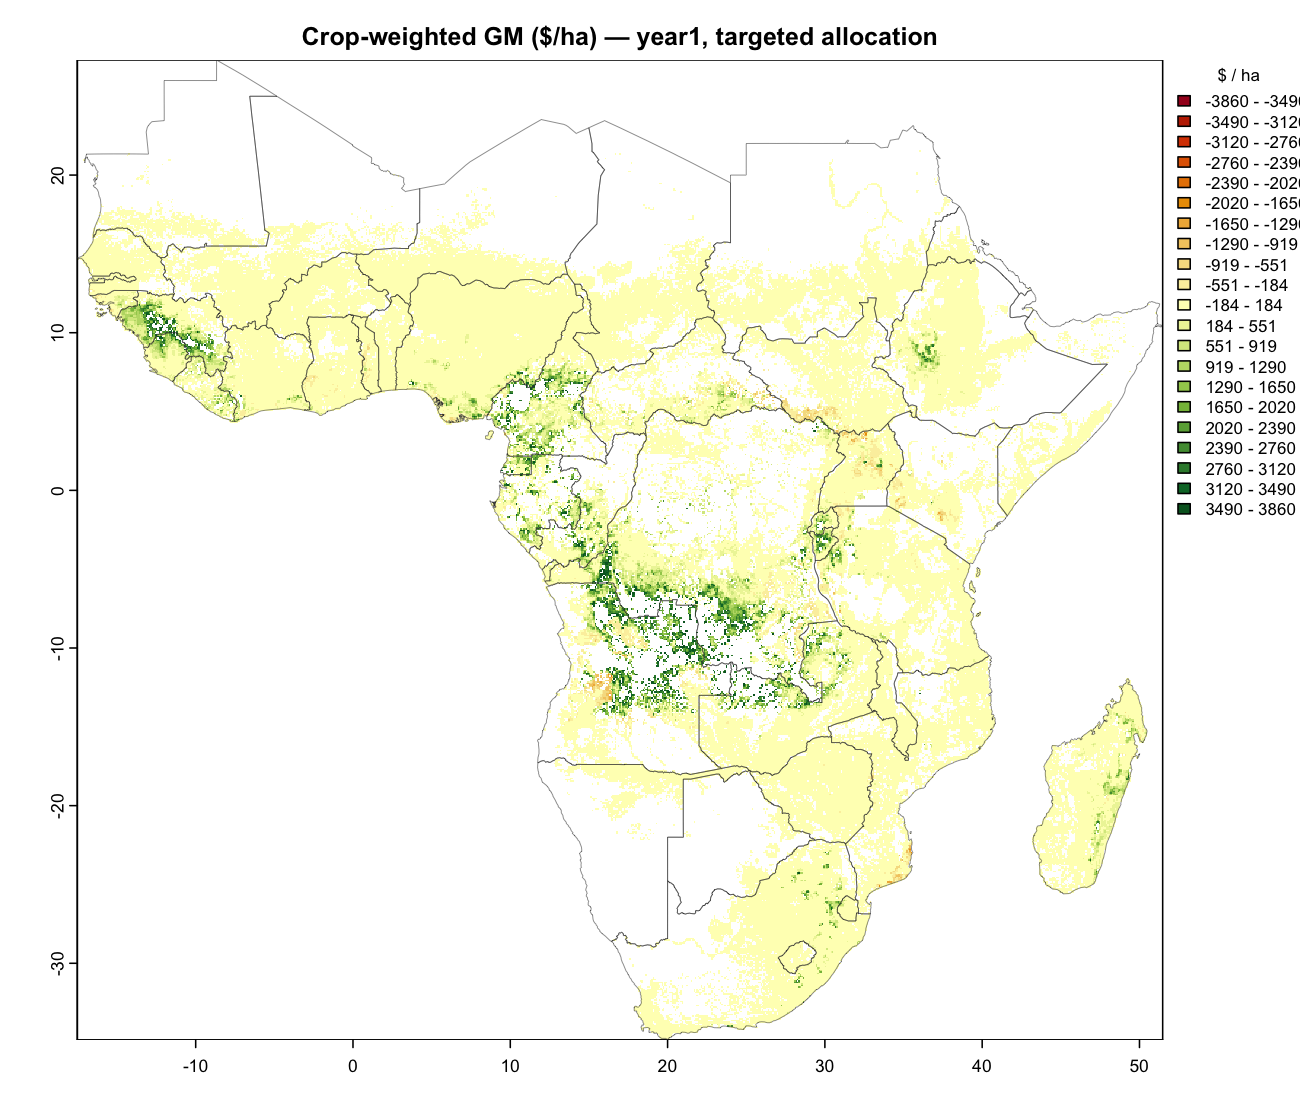
\includegraphics[width=2in,height=\textheight,keepaspectratio]{maps/profitability/ssa_gm_year1_targeted.png}
&
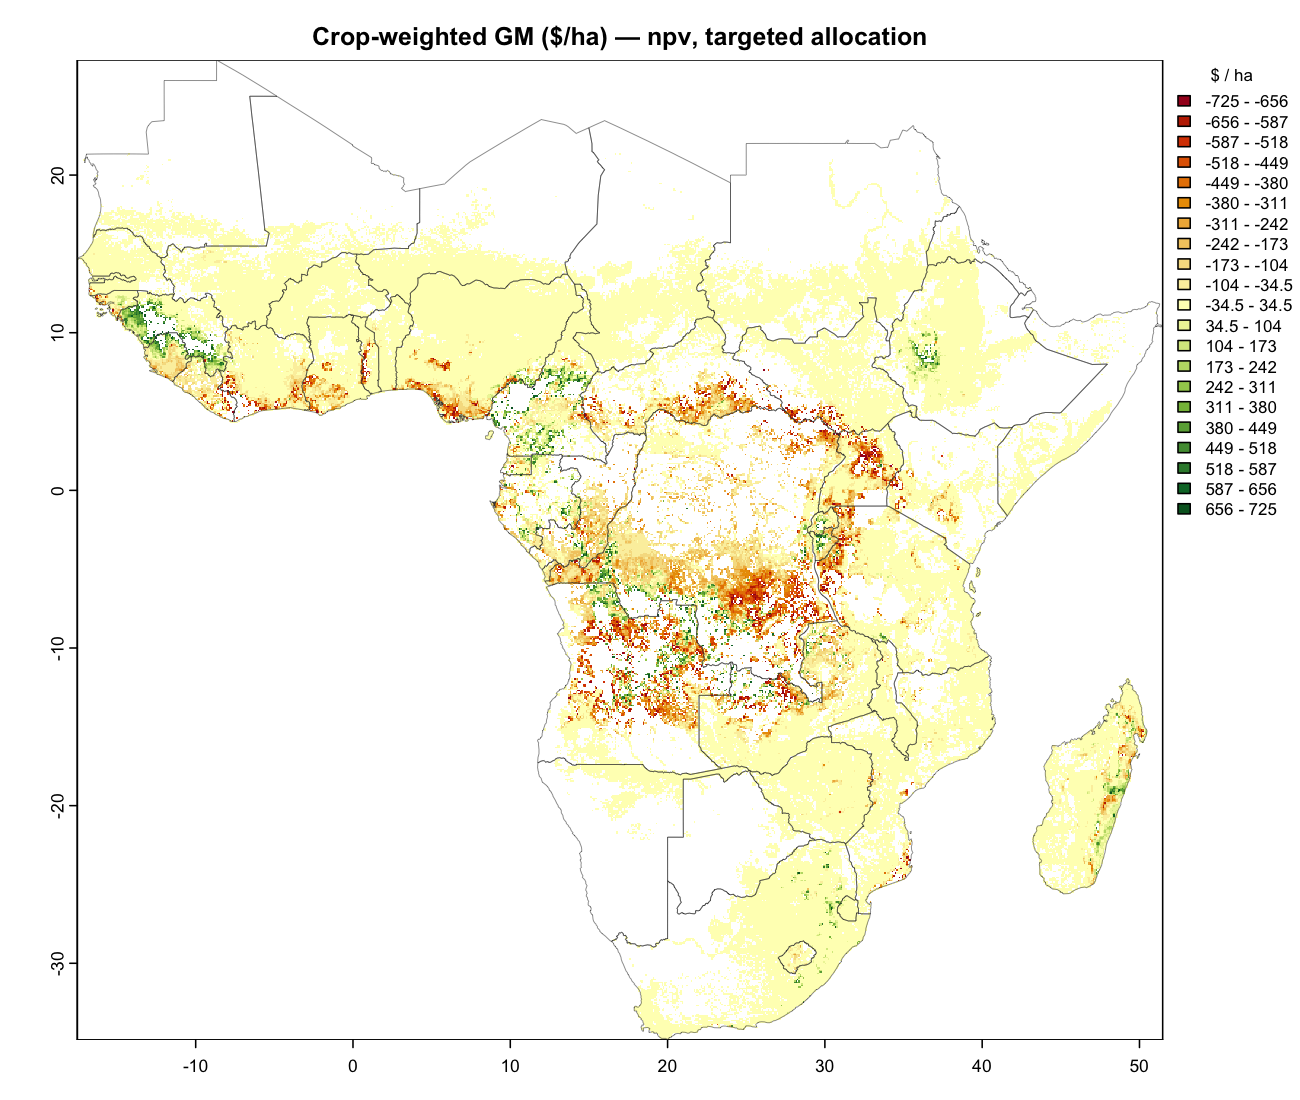
\includegraphics[width=2in,height=\textheight,keepaspectratio]{maps/profitability/ssa_gm_npv_targeted.png}
&
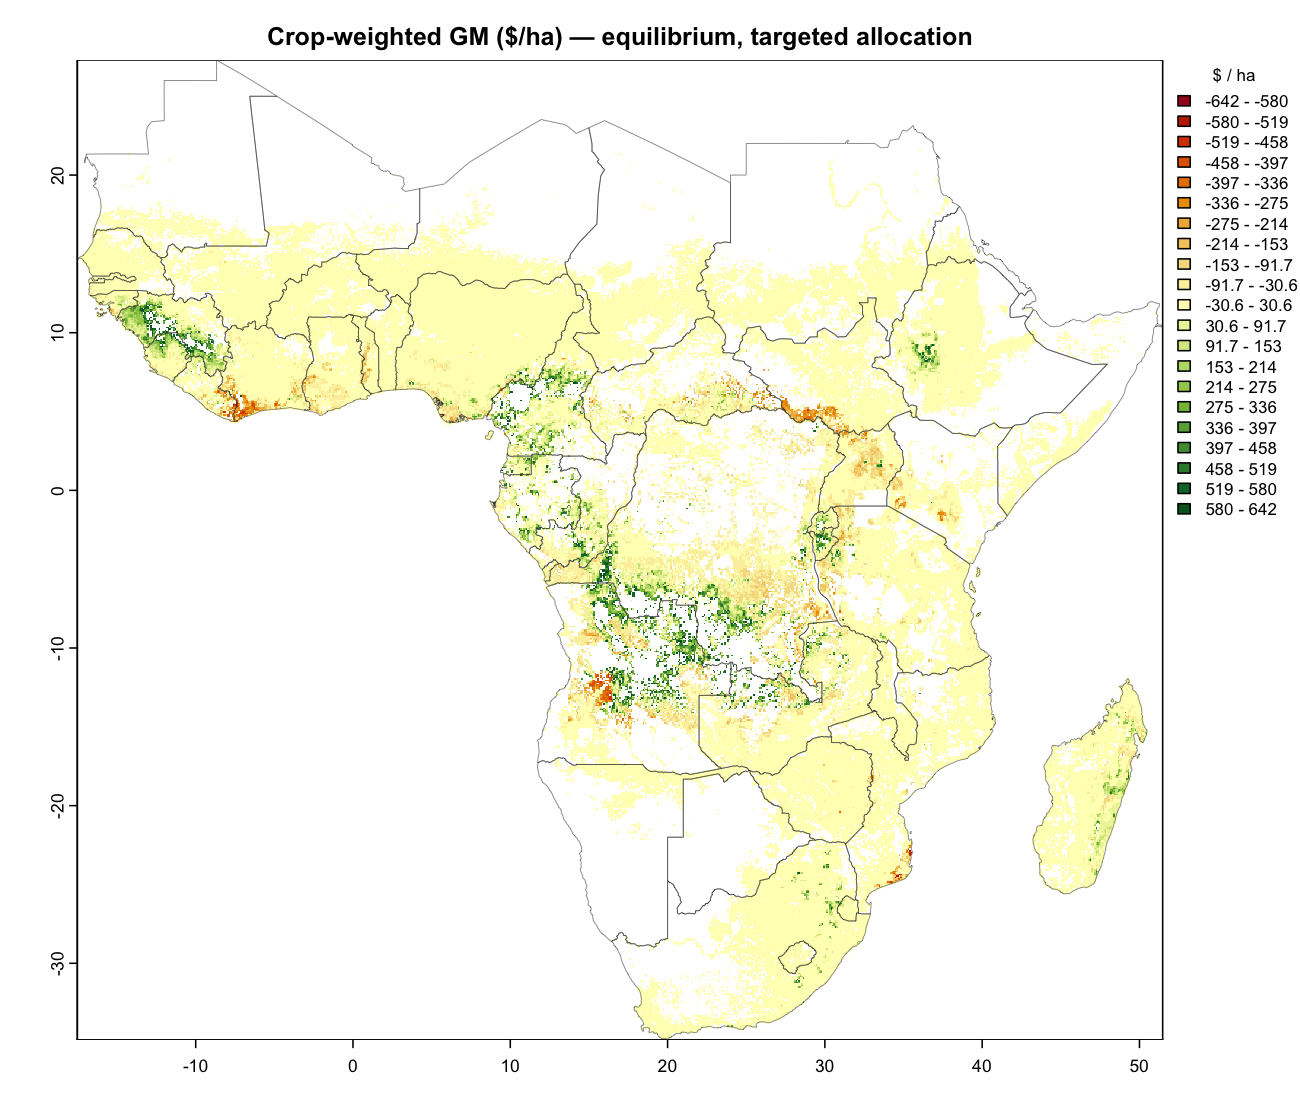
\includegraphics[width=2in,height=\textheight,keepaspectratio]{maps/profitability/ssa_gm_equilibrium_targeted.png} \\
\end{longtable}
}

\subsubsection{1.2 By allocation rule (NPV
regime)}\label{by-allocation-rule-npv-regime}

{\def\LTcaptype{none} % do not increment counter
\begin{longtable}[]{@{}
  >{\centering\arraybackslash}p{(\linewidth - 6\tabcolsep) * \real{0.2500}}
  >{\centering\arraybackslash}p{(\linewidth - 6\tabcolsep) * \real{0.2500}}
  >{\centering\arraybackslash}p{(\linewidth - 6\tabcolsep) * \real{0.2500}}
  >{\centering\arraybackslash}p{(\linewidth - 6\tabcolsep) * \real{0.2500}}@{}}
\toprule\noalign{}
\begin{minipage}[b]{\linewidth}\centering
Targeted
\end{minipage} & \begin{minipage}[b]{\linewidth}\centering
Uniform 10 t/ha
\end{minipage} & \begin{minipage}[b]{\linewidth}\centering
Uniform 20 t/ha
\end{minipage} & \begin{minipage}[b]{\linewidth}\centering
Uniform 50 t/ha
\end{minipage} \\
\midrule\noalign{}
\endhead
\bottomrule\noalign{}
\endlastfoot
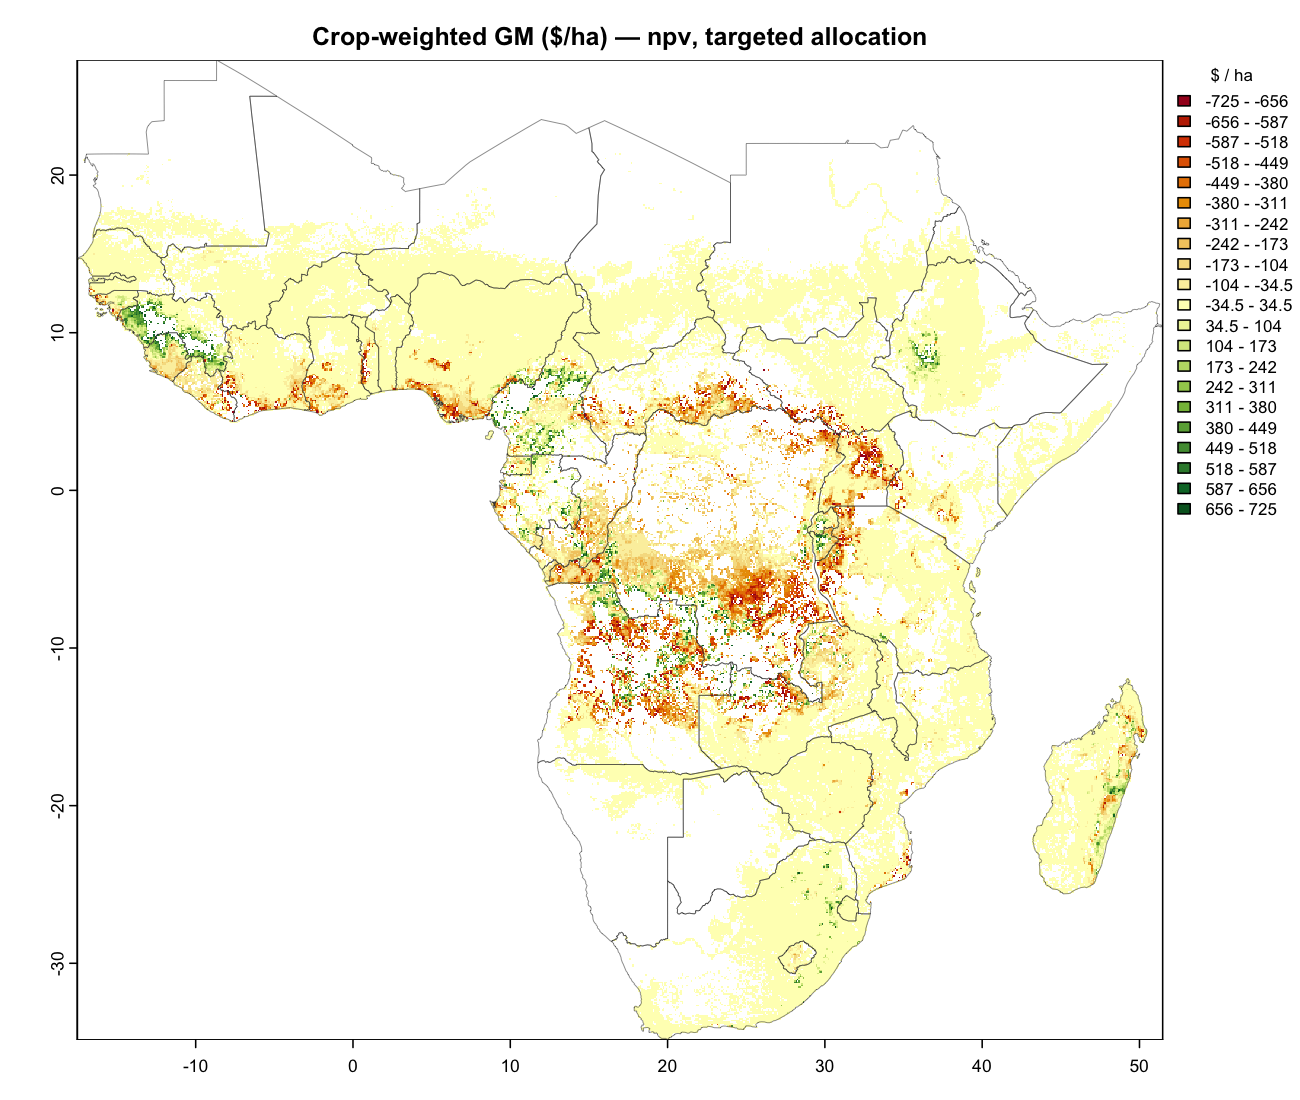
\includegraphics[width=1.6in,height=\textheight,keepaspectratio]{maps/profitability/ssa_gm_npv_targeted.png}
&
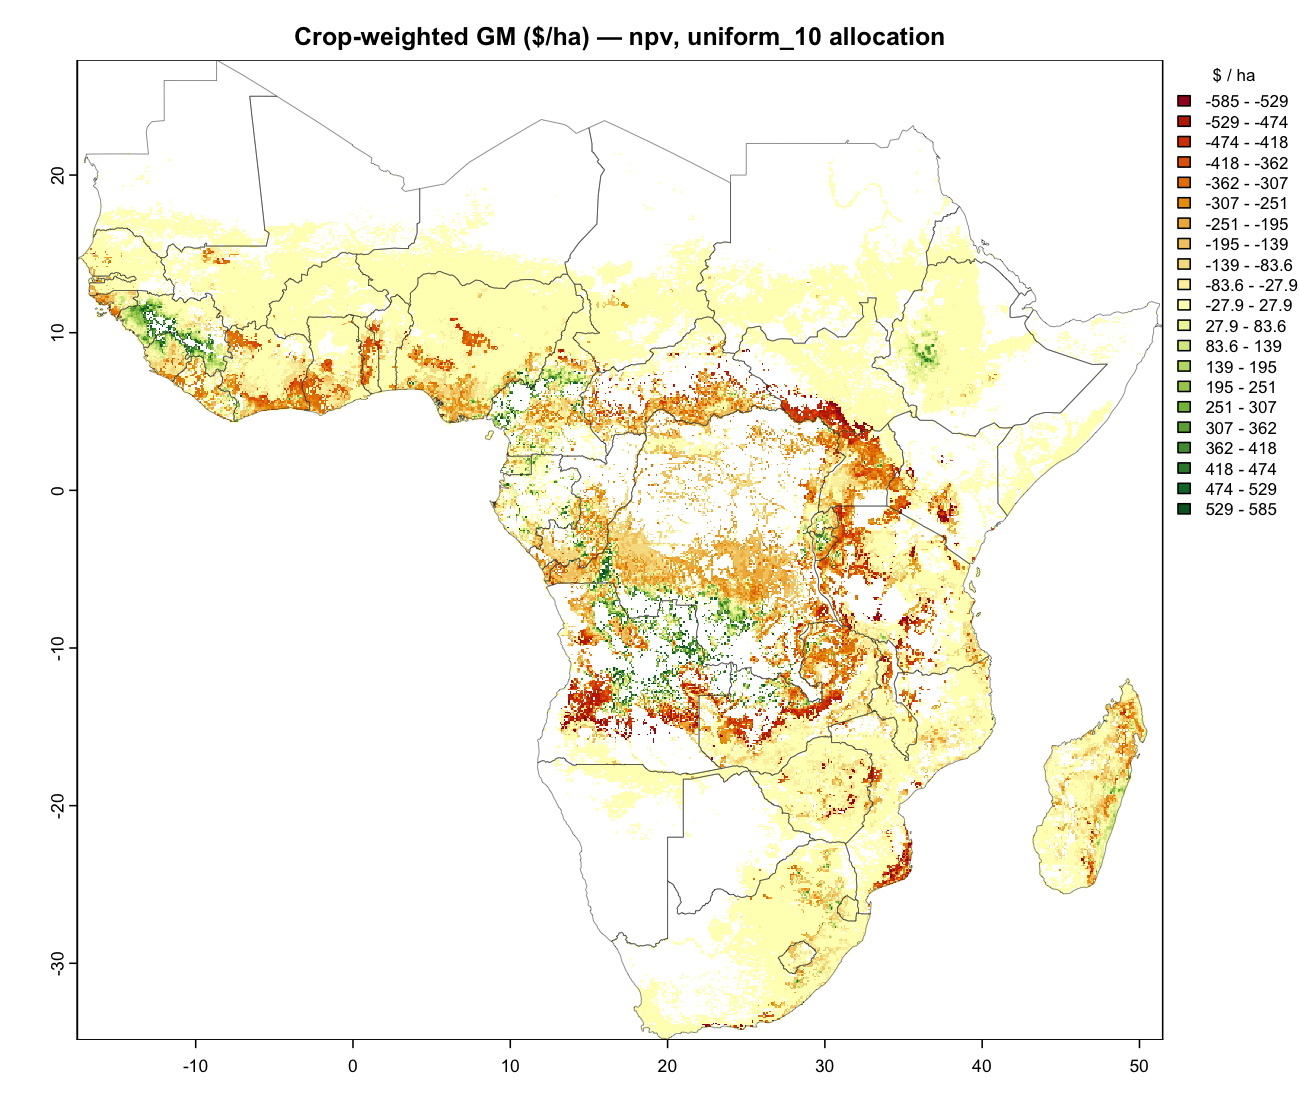
\includegraphics[width=1.6in,height=\textheight,keepaspectratio]{maps/profitability/ssa_gm_npv_uniform_10.png}
&
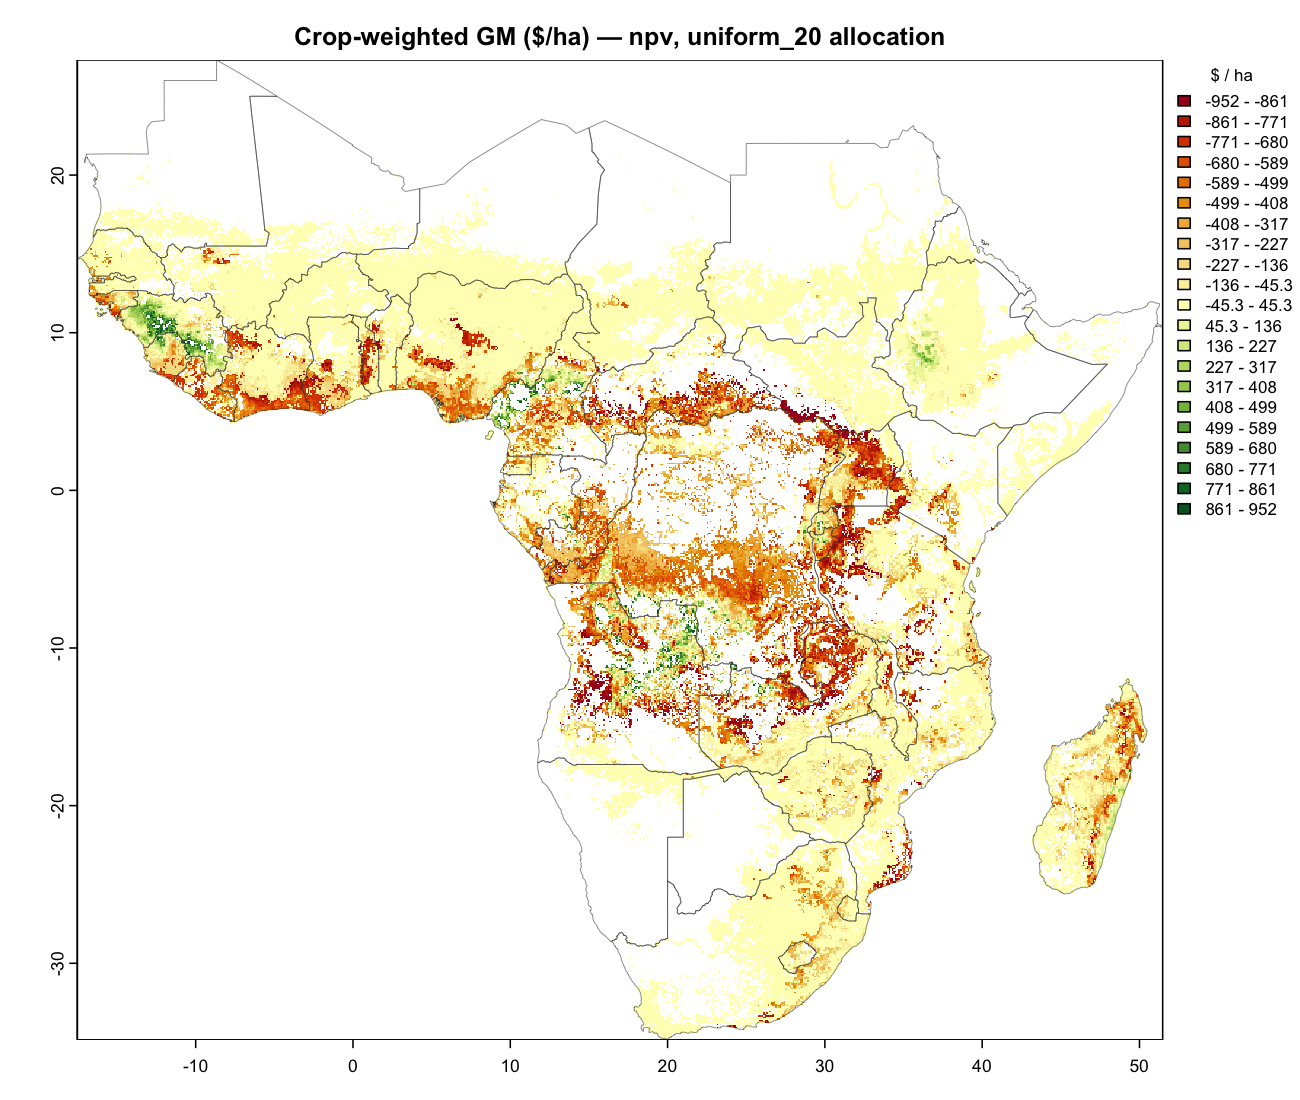
\includegraphics[width=1.6in,height=\textheight,keepaspectratio]{maps/profitability/ssa_gm_npv_uniform_20.png}
&
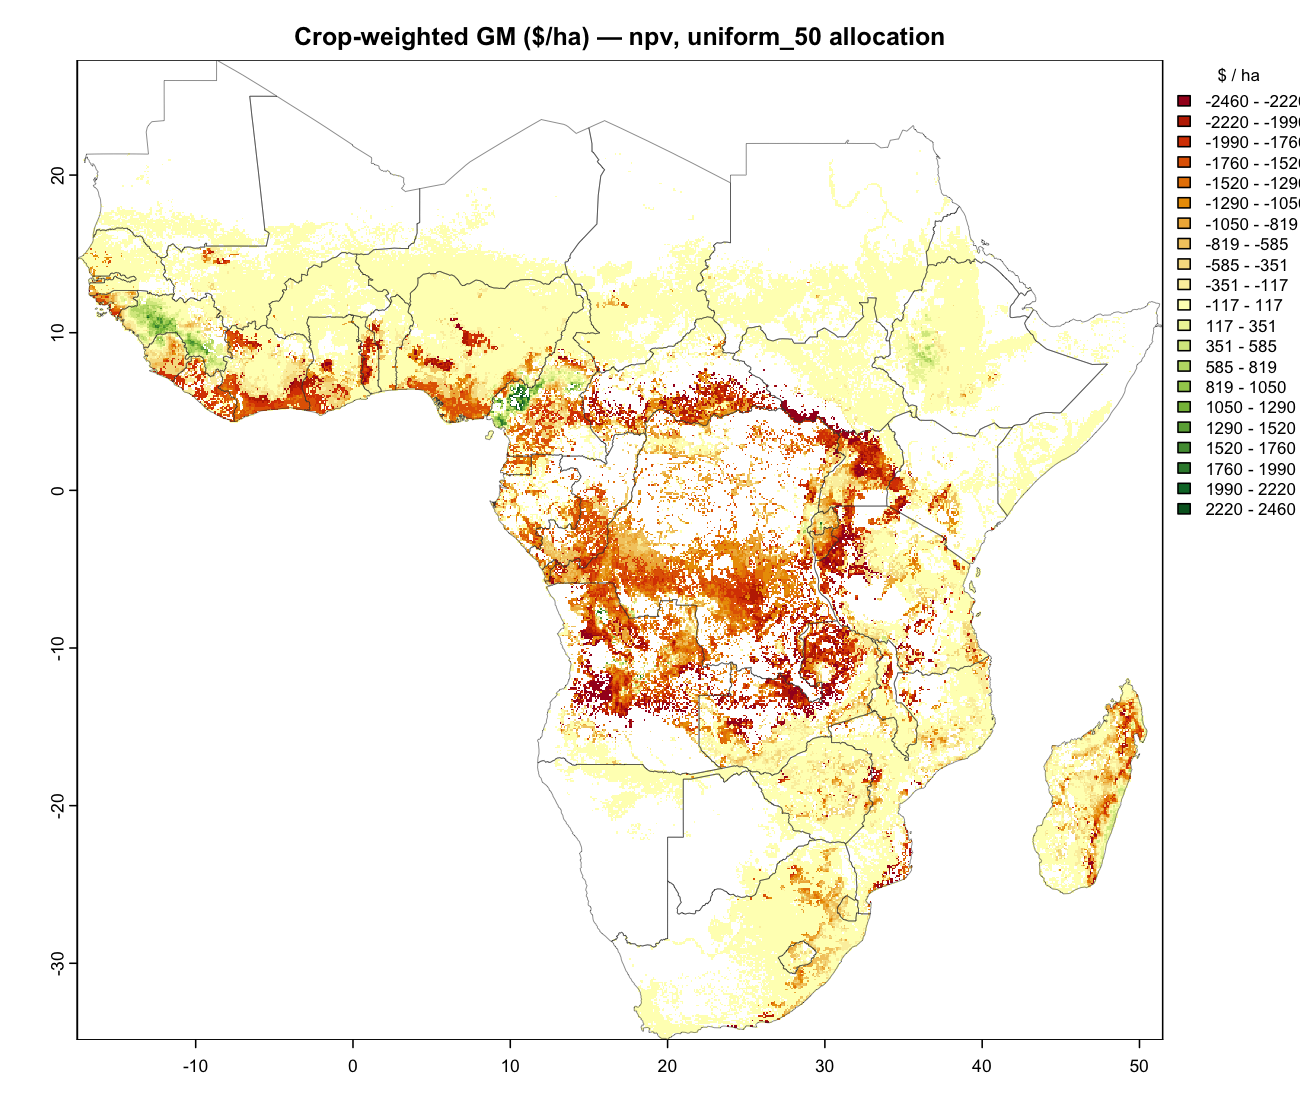
\includegraphics[width=1.6in,height=\textheight,keepaspectratio]{maps/profitability/ssa_gm_npv_uniform_50.png} \\
\end{longtable}
}

The targeted allocation prunes the action set to acidic pixels and pays
the LiTAS-calibrated dose; uniform rules pay a fixed rate across all
cropland and recover CDR even on near-neutral soils that the targeted
rule skips.

\begin{center}\rule{0.5\linewidth}{0.5pt}\end{center}

\subsection{2. Profitable footprint}\label{profitable-footprint}

Binary masks showing where the crop-weighted GM is strictly positive.
These are the candidate pixels for the supply-ranked deployment in
\texttt{erw-supply}.

{\def\LTcaptype{none} % do not increment counter
\begin{longtable}[]{@{}
  >{\raggedright\arraybackslash}p{(\linewidth - 8\tabcolsep) * \real{0.2000}}
  >{\centering\arraybackslash}p{(\linewidth - 8\tabcolsep) * \real{0.2000}}
  >{\centering\arraybackslash}p{(\linewidth - 8\tabcolsep) * \real{0.2000}}
  >{\centering\arraybackslash}p{(\linewidth - 8\tabcolsep) * \real{0.2000}}
  >{\centering\arraybackslash}p{(\linewidth - 8\tabcolsep) * \real{0.2000}}@{}}
\toprule\noalign{}
\begin{minipage}[b]{\linewidth}\raggedright
\end{minipage} & \begin{minipage}[b]{\linewidth}\centering
Targeted
\end{minipage} & \begin{minipage}[b]{\linewidth}\centering
Uniform 10
\end{minipage} & \begin{minipage}[b]{\linewidth}\centering
Uniform 20
\end{minipage} & \begin{minipage}[b]{\linewidth}\centering
Uniform 50
\end{minipage} \\
\midrule\noalign{}
\endhead
\bottomrule\noalign{}
\endlastfoot
Year-1 &
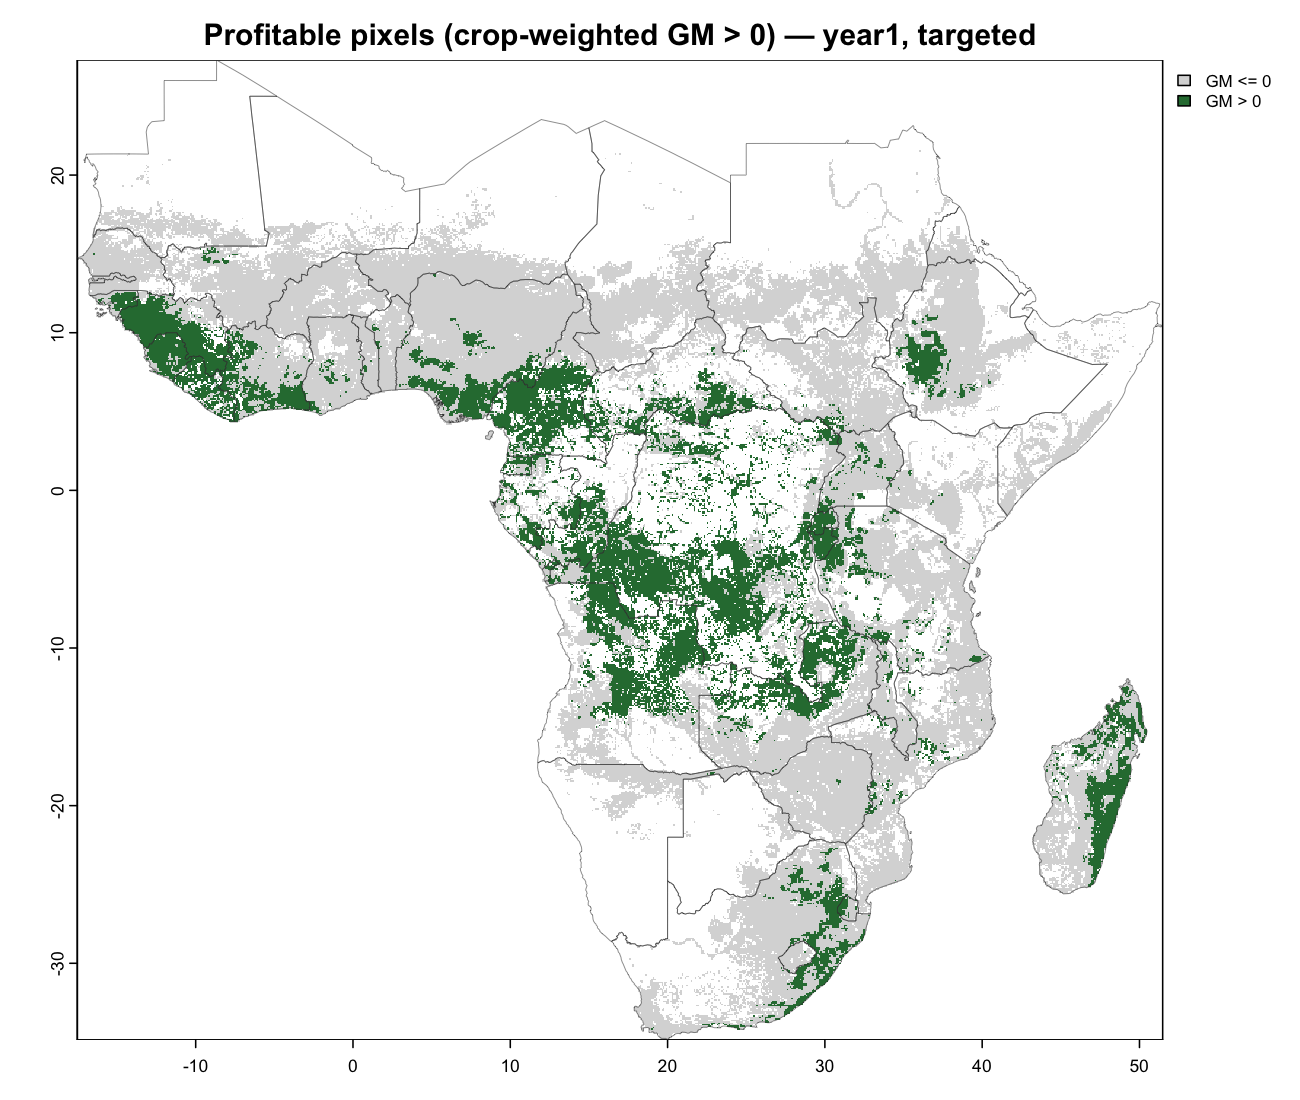
\includegraphics[width=1.4in,height=\textheight,keepaspectratio]{maps/profitability/profitable_mask_year1_targeted.png}
&
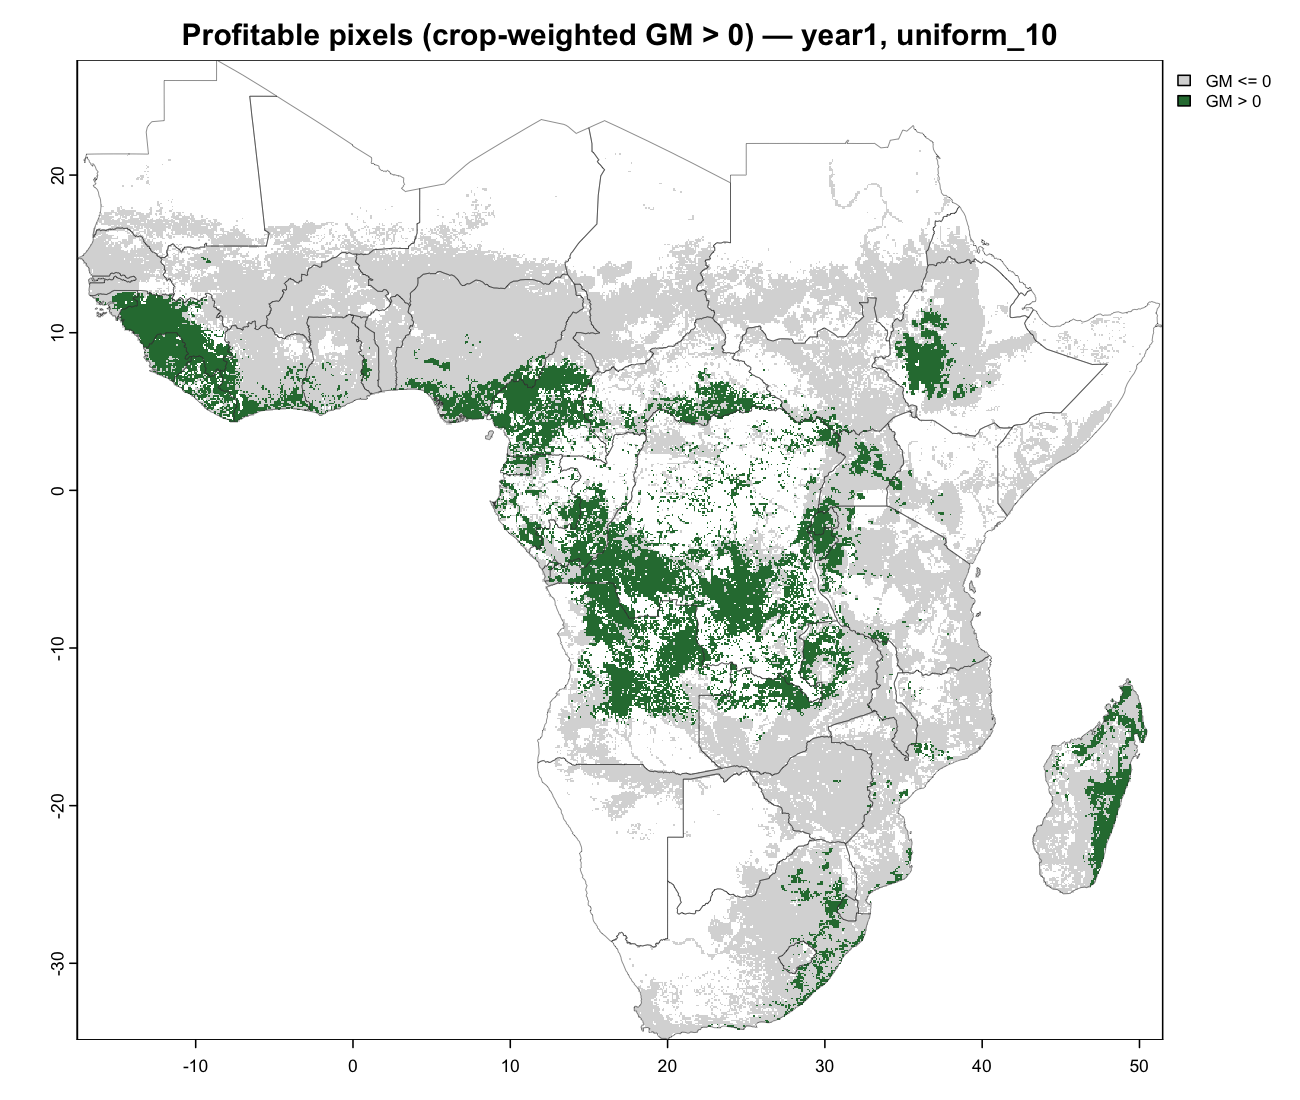
\includegraphics[width=1.4in,height=\textheight,keepaspectratio]{maps/profitability/profitable_mask_year1_uniform_10.png}
&
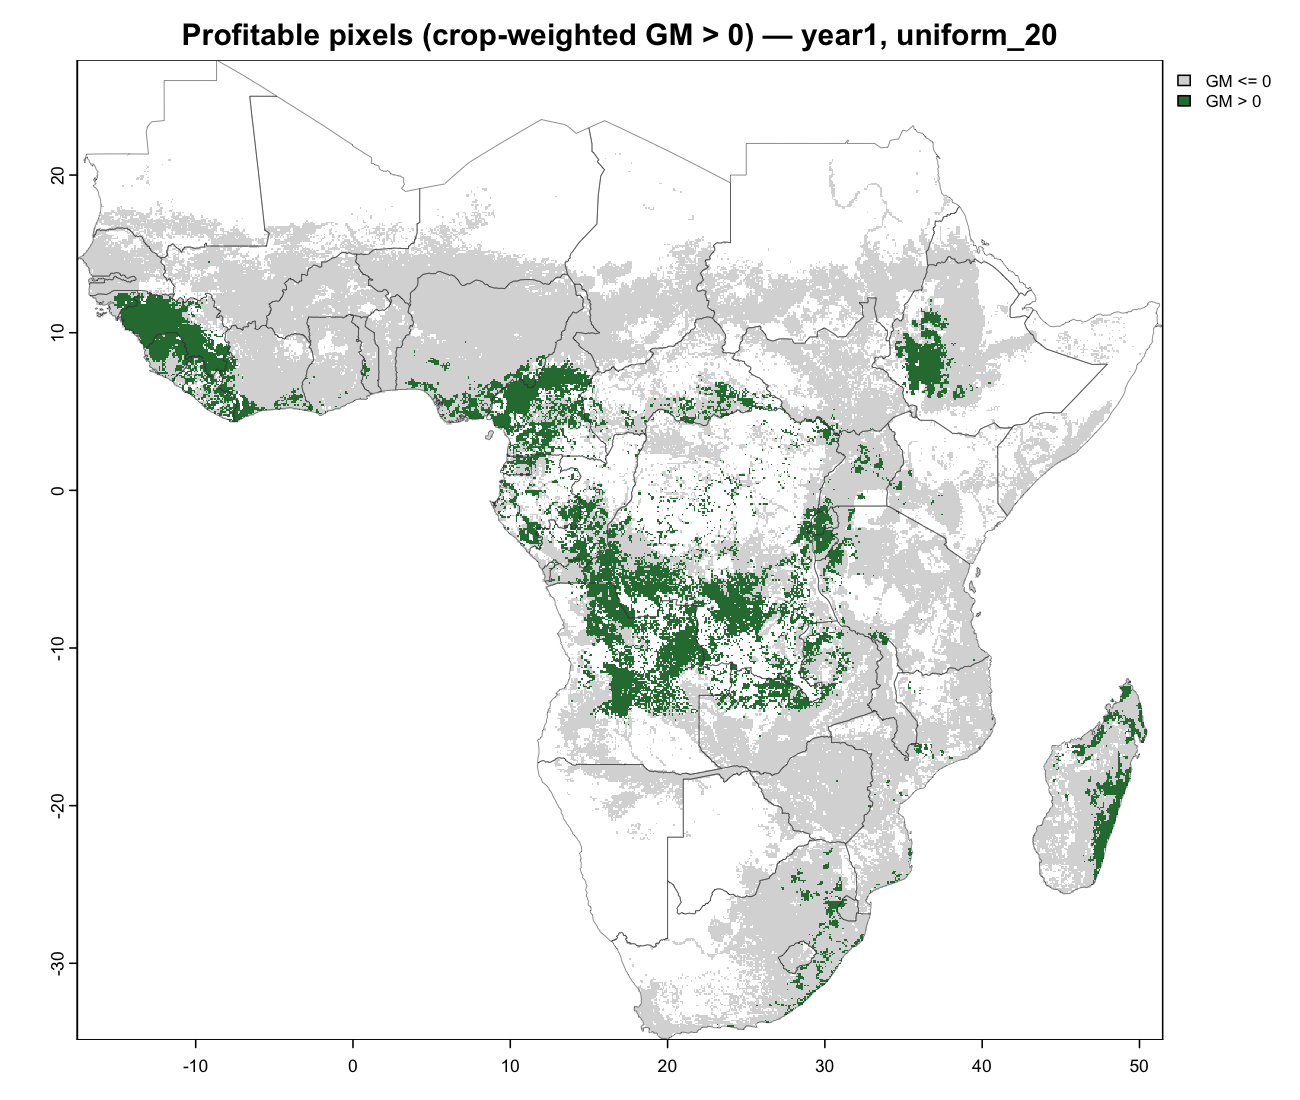
\includegraphics[width=1.4in,height=\textheight,keepaspectratio]{maps/profitability/profitable_mask_year1_uniform_20.png}
&
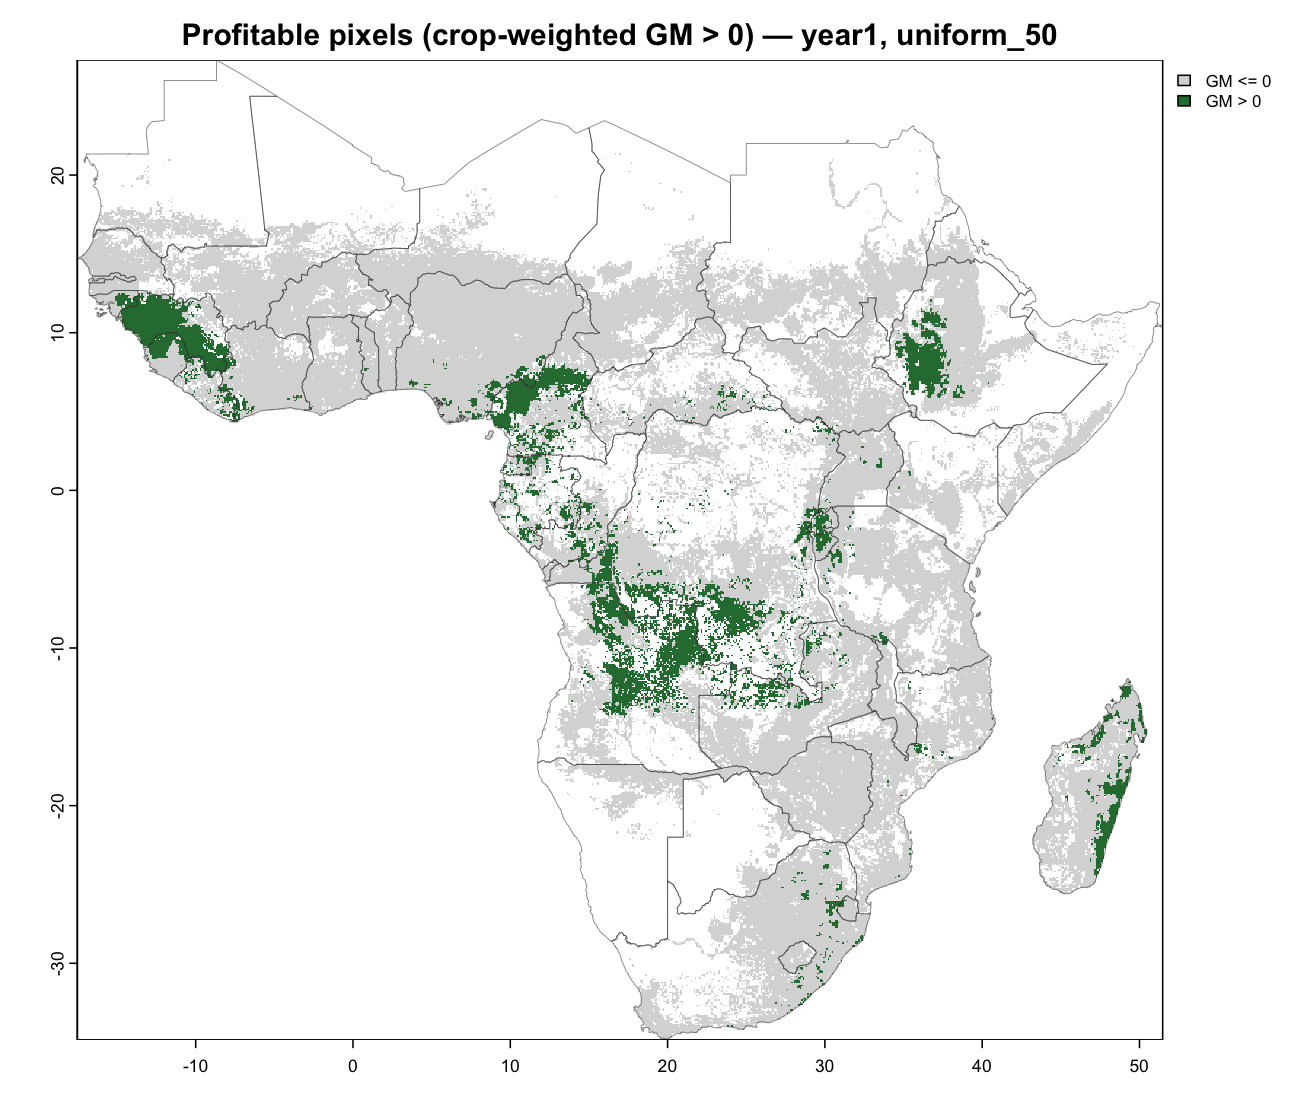
\includegraphics[width=1.4in,height=\textheight,keepaspectratio]{maps/profitability/profitable_mask_year1_uniform_50.png} \\
NPV &
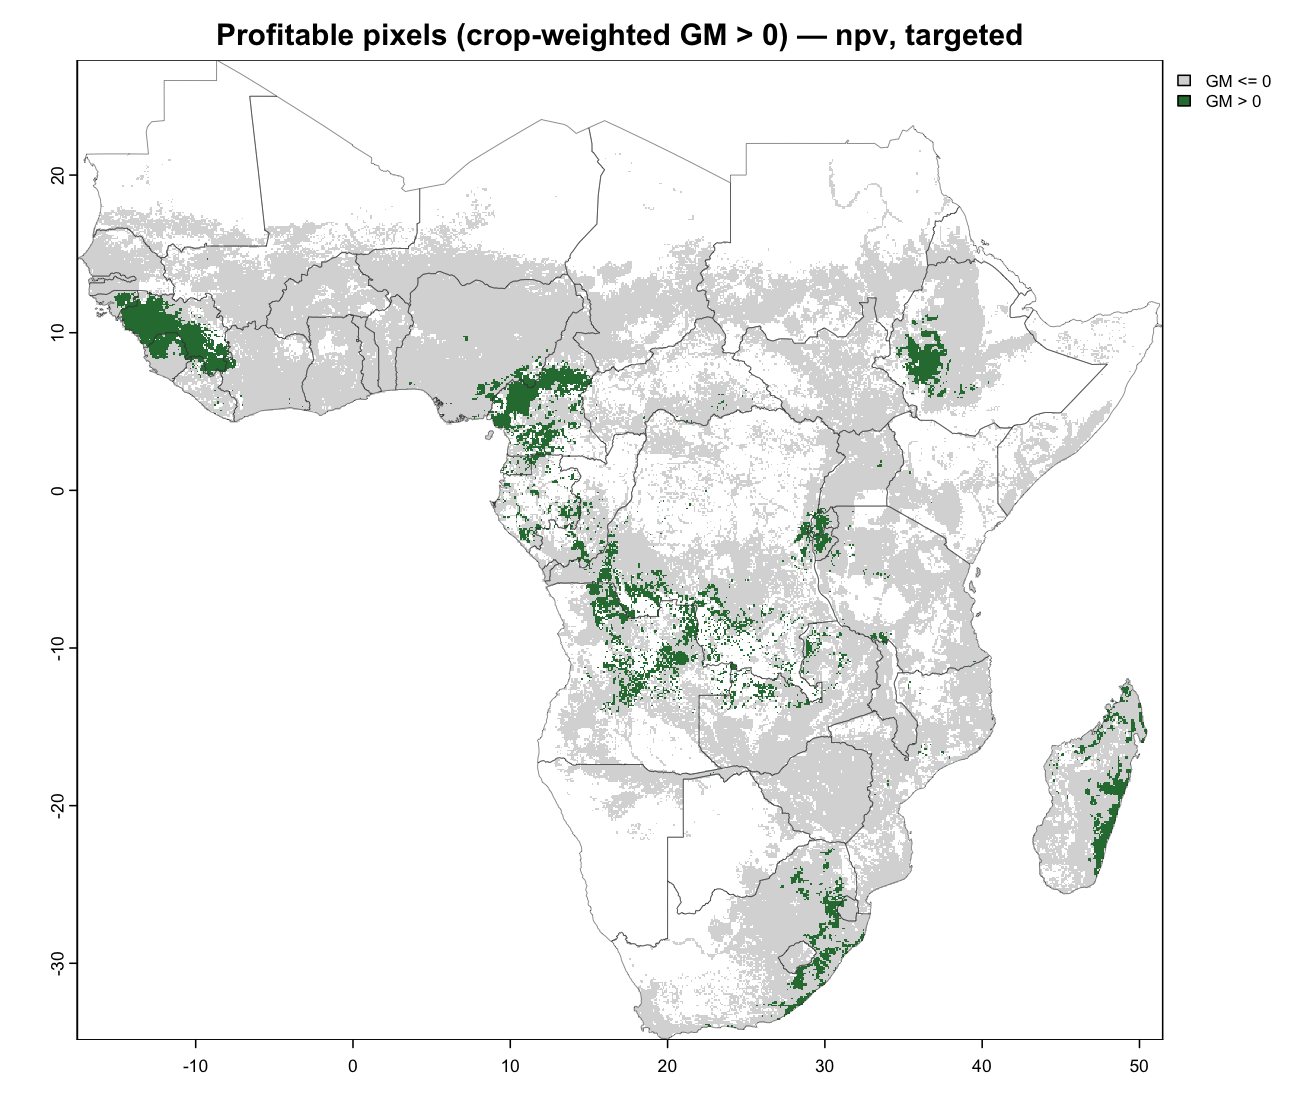
\includegraphics[width=1.4in,height=\textheight,keepaspectratio]{maps/profitability/profitable_mask_npv_targeted.png}
&
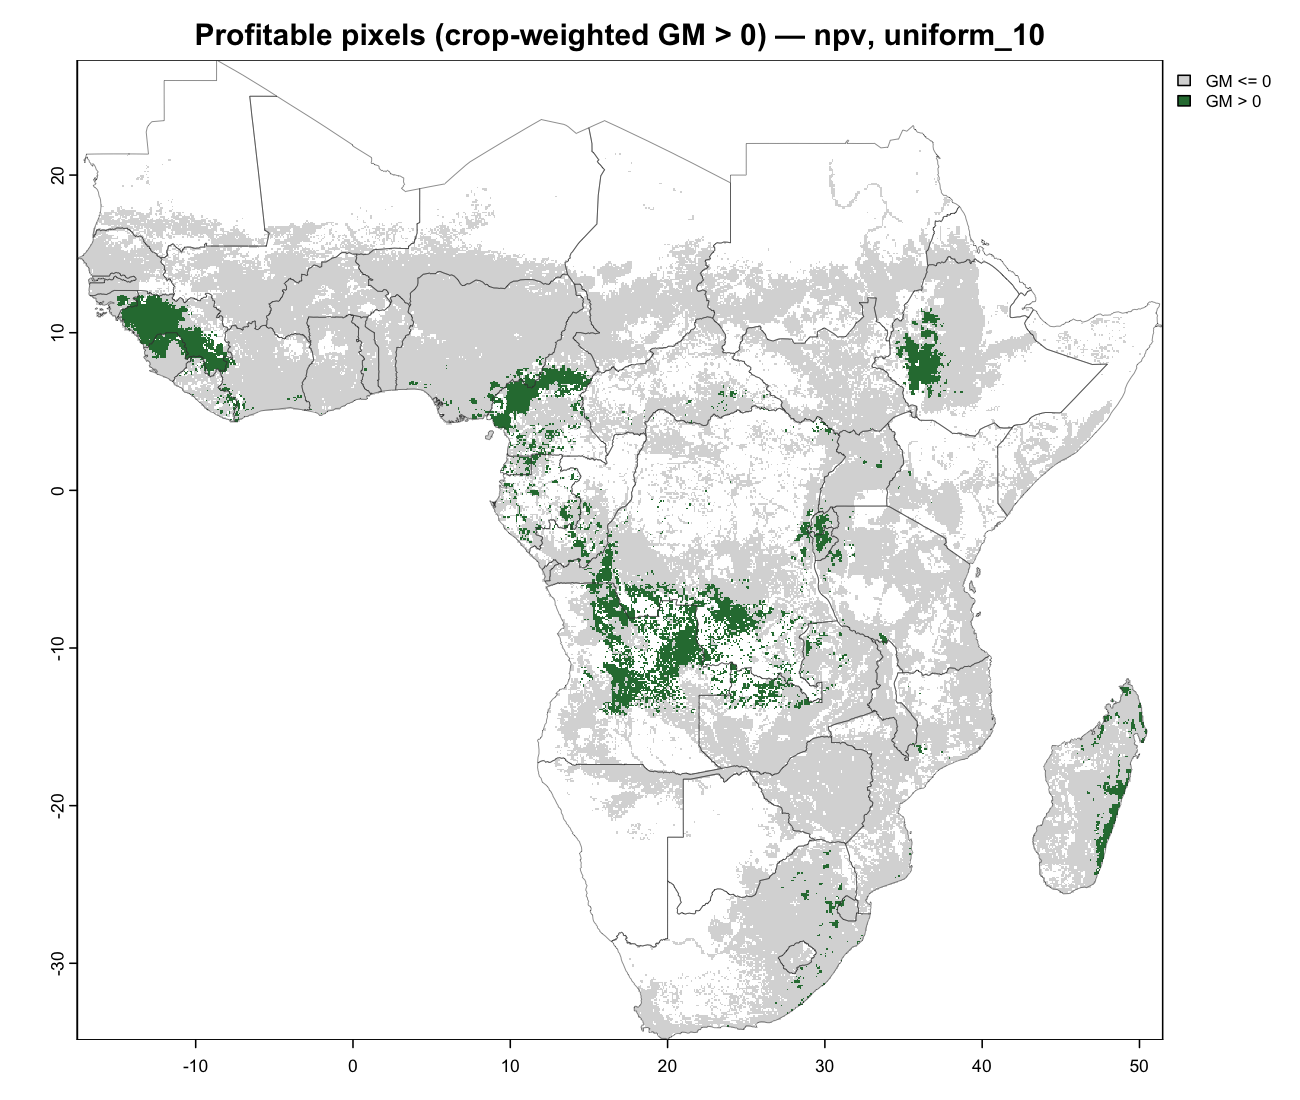
\includegraphics[width=1.4in,height=\textheight,keepaspectratio]{maps/profitability/profitable_mask_npv_uniform_10.png}
&
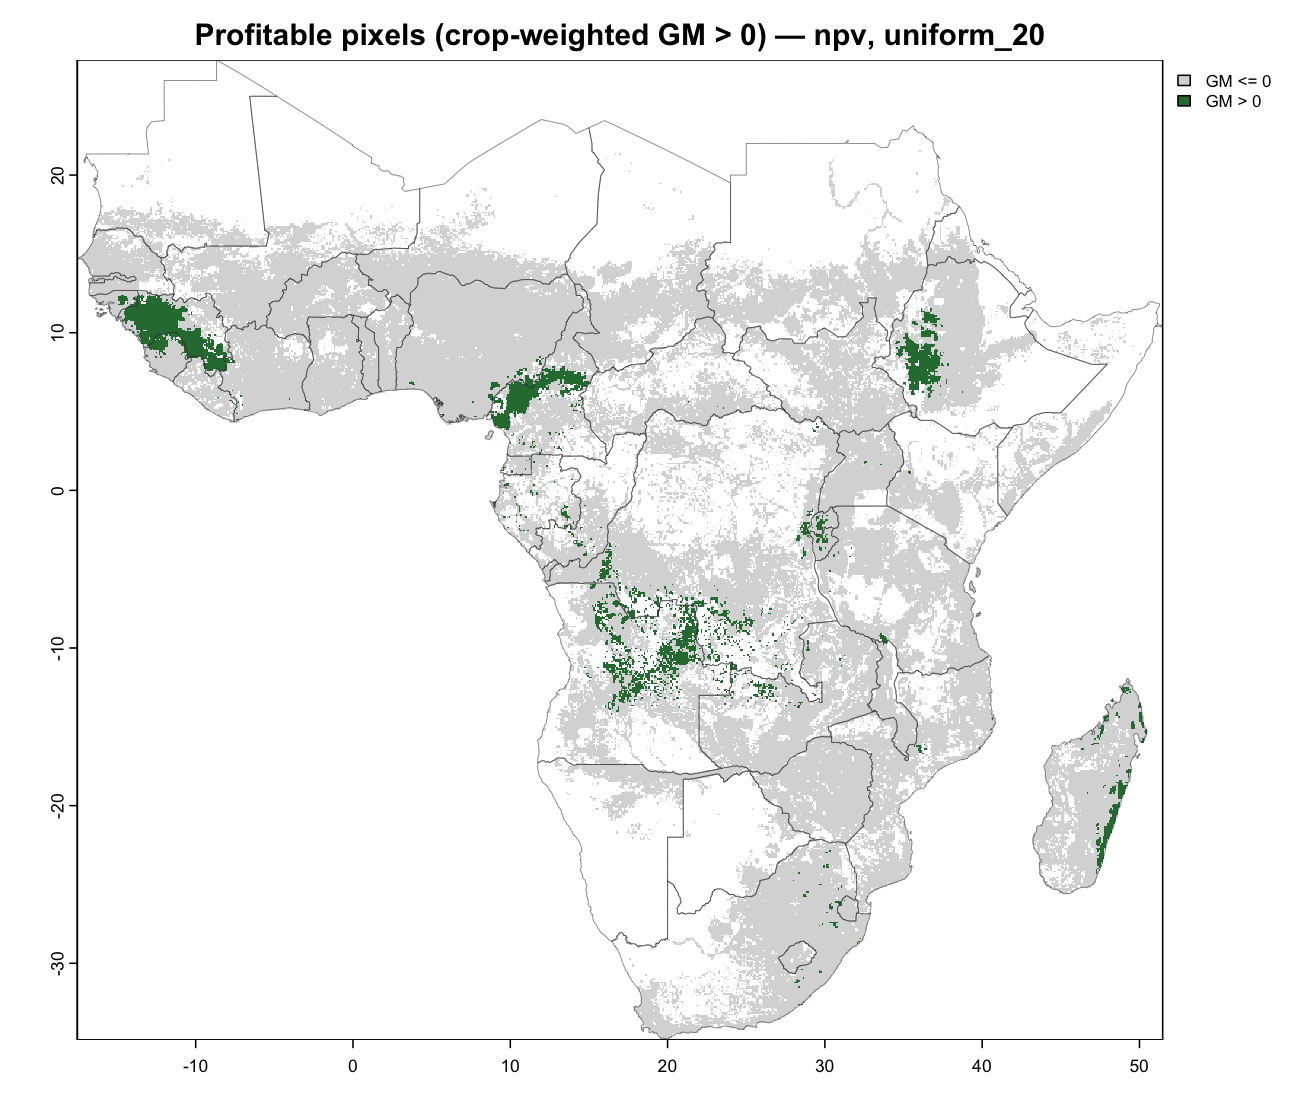
\includegraphics[width=1.4in,height=\textheight,keepaspectratio]{maps/profitability/profitable_mask_npv_uniform_20.png}
&
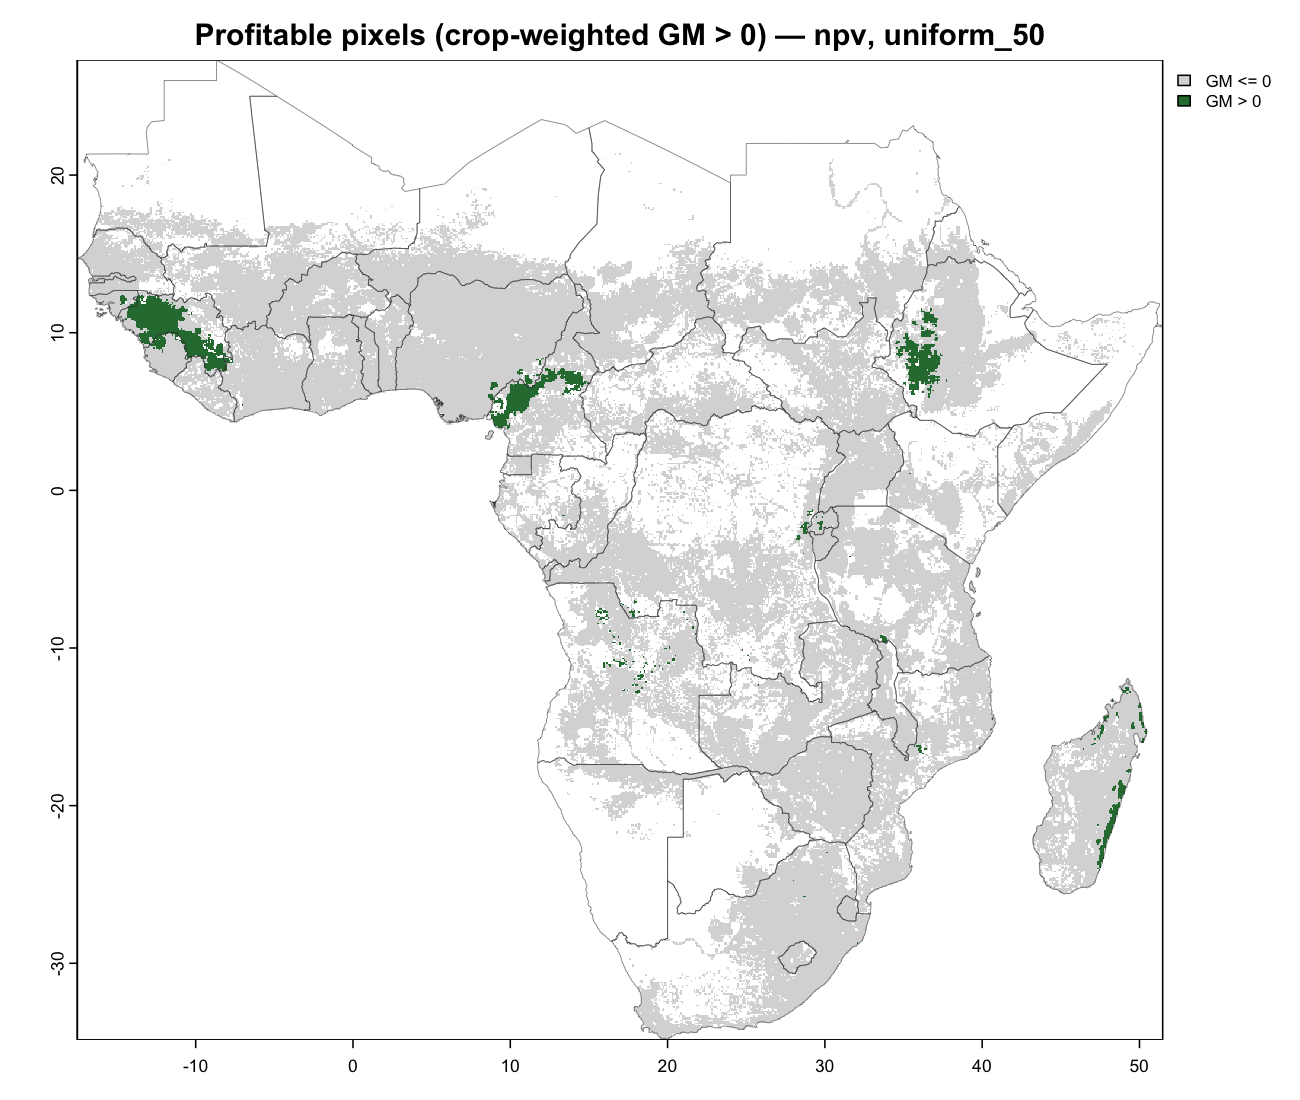
\includegraphics[width=1.4in,height=\textheight,keepaspectratio]{maps/profitability/profitable_mask_npv_uniform_50.png} \\
Equilibrium &
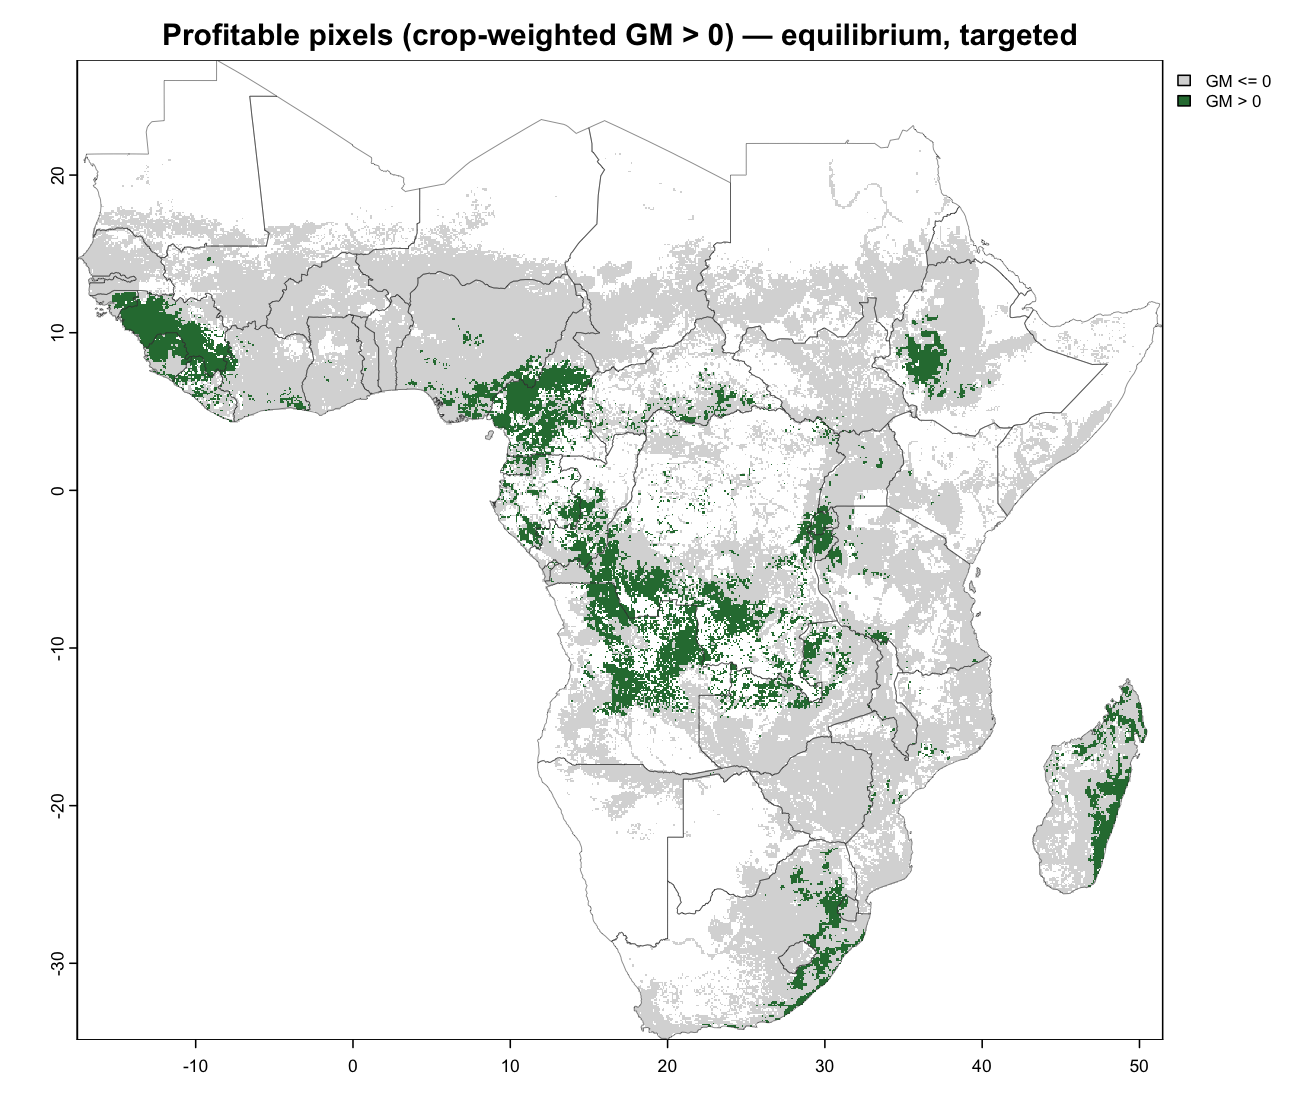
\includegraphics[width=1.4in,height=\textheight,keepaspectratio]{maps/profitability/profitable_mask_equilibrium_targeted.png}
&
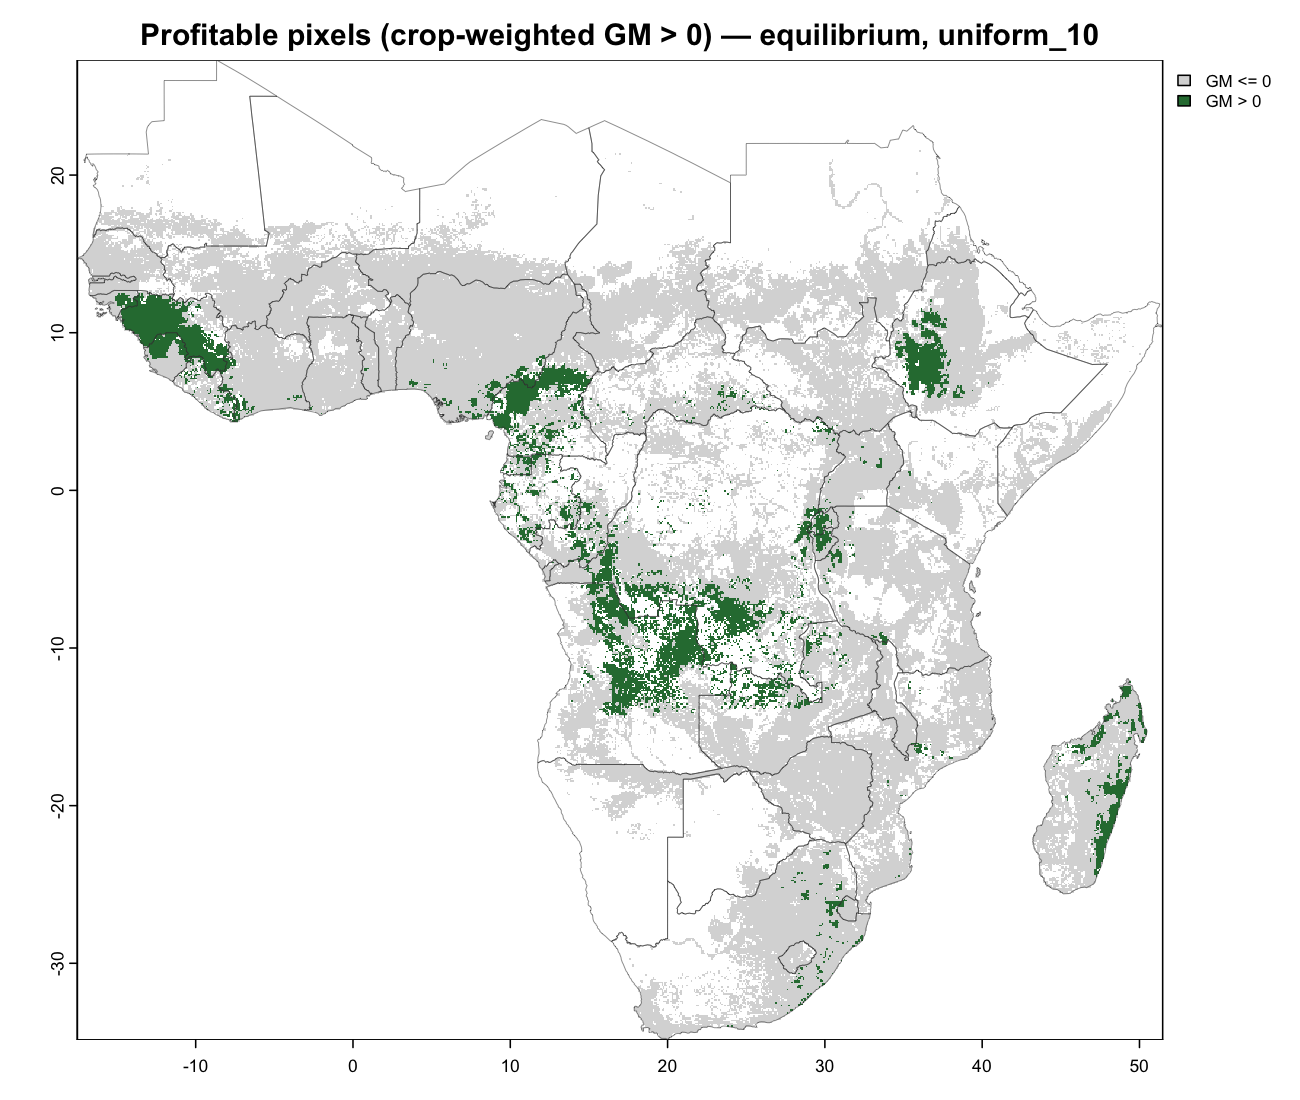
\includegraphics[width=1.4in,height=\textheight,keepaspectratio]{maps/profitability/profitable_mask_equilibrium_uniform_10.png}
&
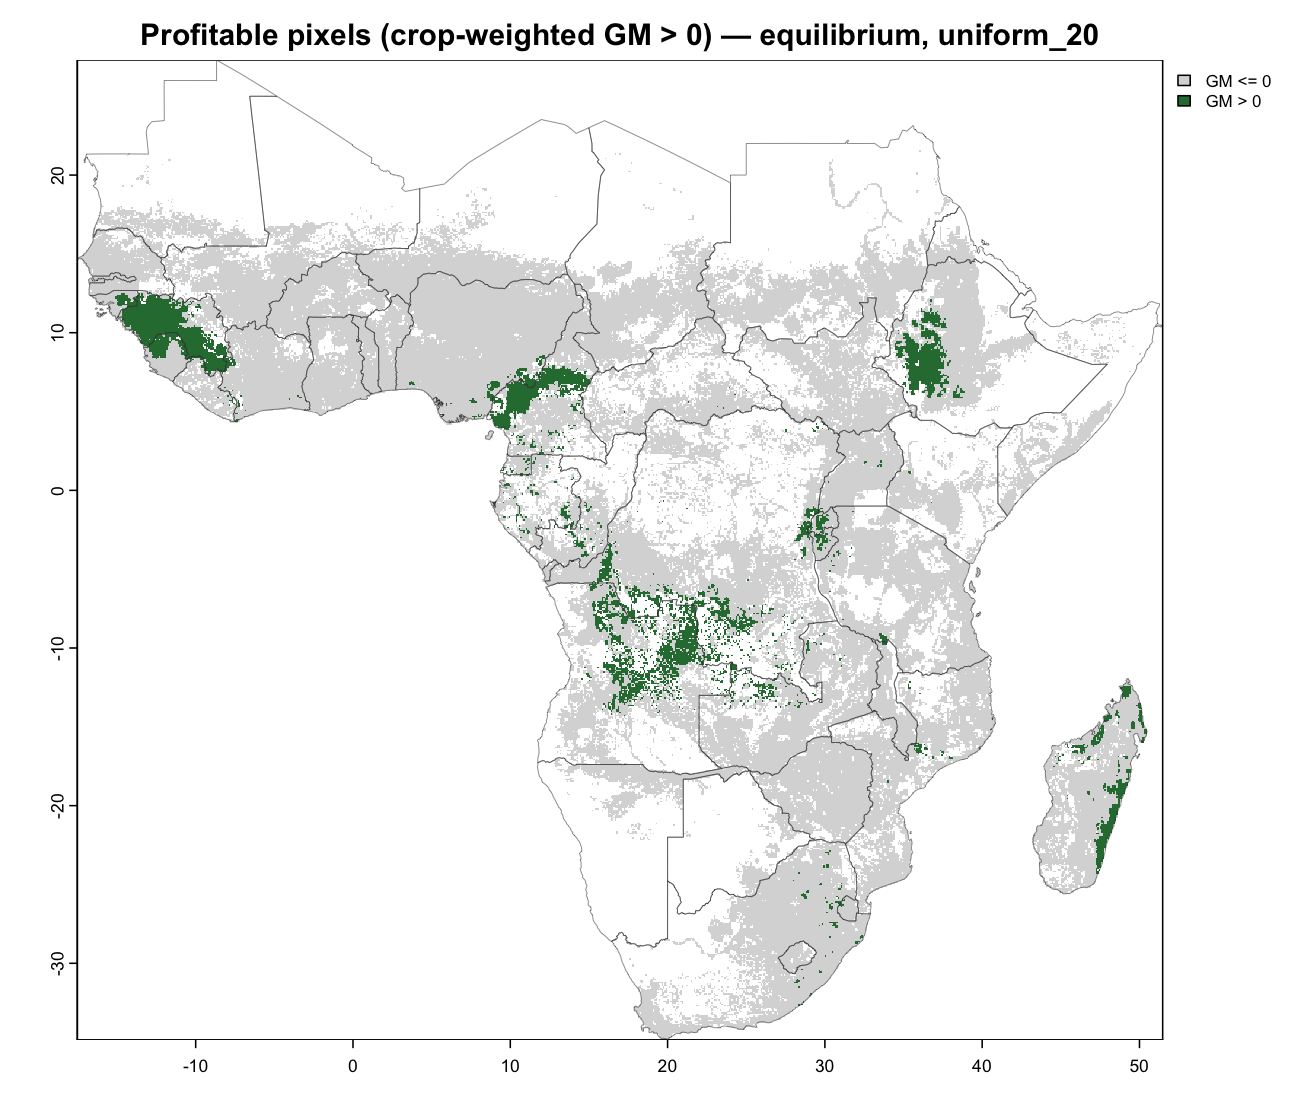
\includegraphics[width=1.4in,height=\textheight,keepaspectratio]{maps/profitability/profitable_mask_equilibrium_uniform_20.png}
&
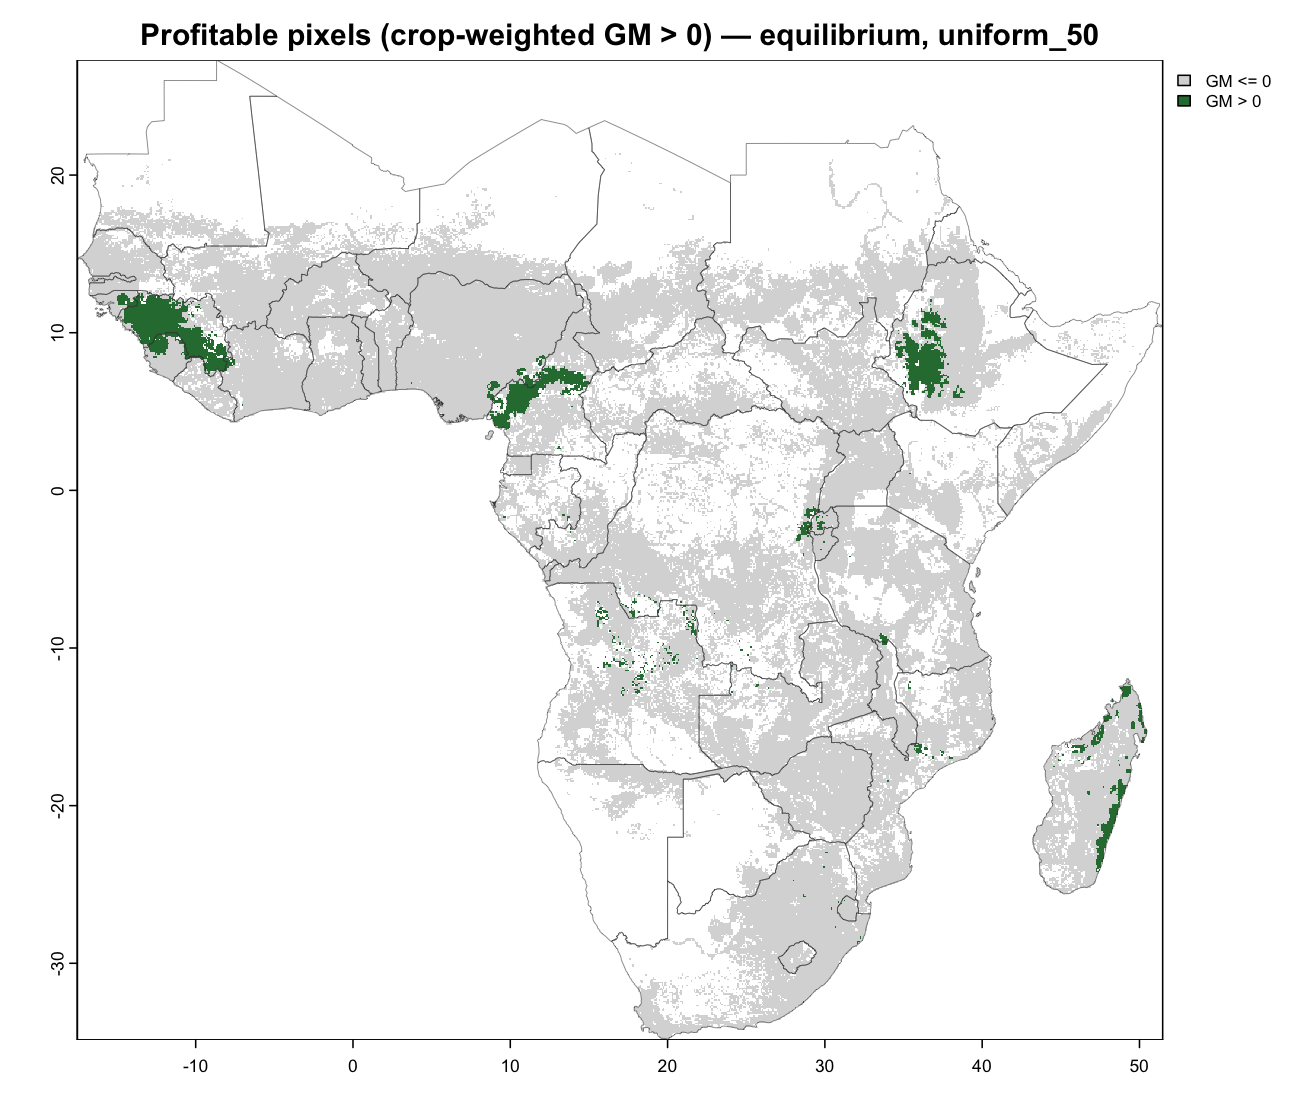
\includegraphics[width=1.4in,height=\textheight,keepaspectratio]{maps/profitability/profitable_mask_equilibrium_uniform_50.png} \\
\end{longtable}
}

\begin{center}\rule{0.5\linewidth}{0.5pt}\end{center}

\subsection{3. Breakeven carbon price}\label{breakeven-carbon-price}

For each pixel, the minimum carbon price (\$ / tCO₂) that drives
crop-weighted GM to zero, holding all other defaults constant (MRV \$20
/ tCO₂, grain size 50 µm, etc.). Pixels with no CDR potential are
masked; the legend caps at \$500 / tCO₂ for legibility.

{\def\LTcaptype{none} % do not increment counter
\begin{longtable}[]{@{}
  >{\centering\arraybackslash}p{(\linewidth - 4\tabcolsep) * \real{0.3333}}
  >{\centering\arraybackslash}p{(\linewidth - 4\tabcolsep) * \real{0.3333}}
  >{\centering\arraybackslash}p{(\linewidth - 4\tabcolsep) * \real{0.3333}}@{}}
\toprule\noalign{}
\begin{minipage}[b]{\linewidth}\centering
Year-1
\end{minipage} & \begin{minipage}[b]{\linewidth}\centering
NPV @ 10 \%
\end{minipage} & \begin{minipage}[b]{\linewidth}\centering
Equilibrium
\end{minipage} \\
\midrule\noalign{}
\endhead
\bottomrule\noalign{}
\endlastfoot
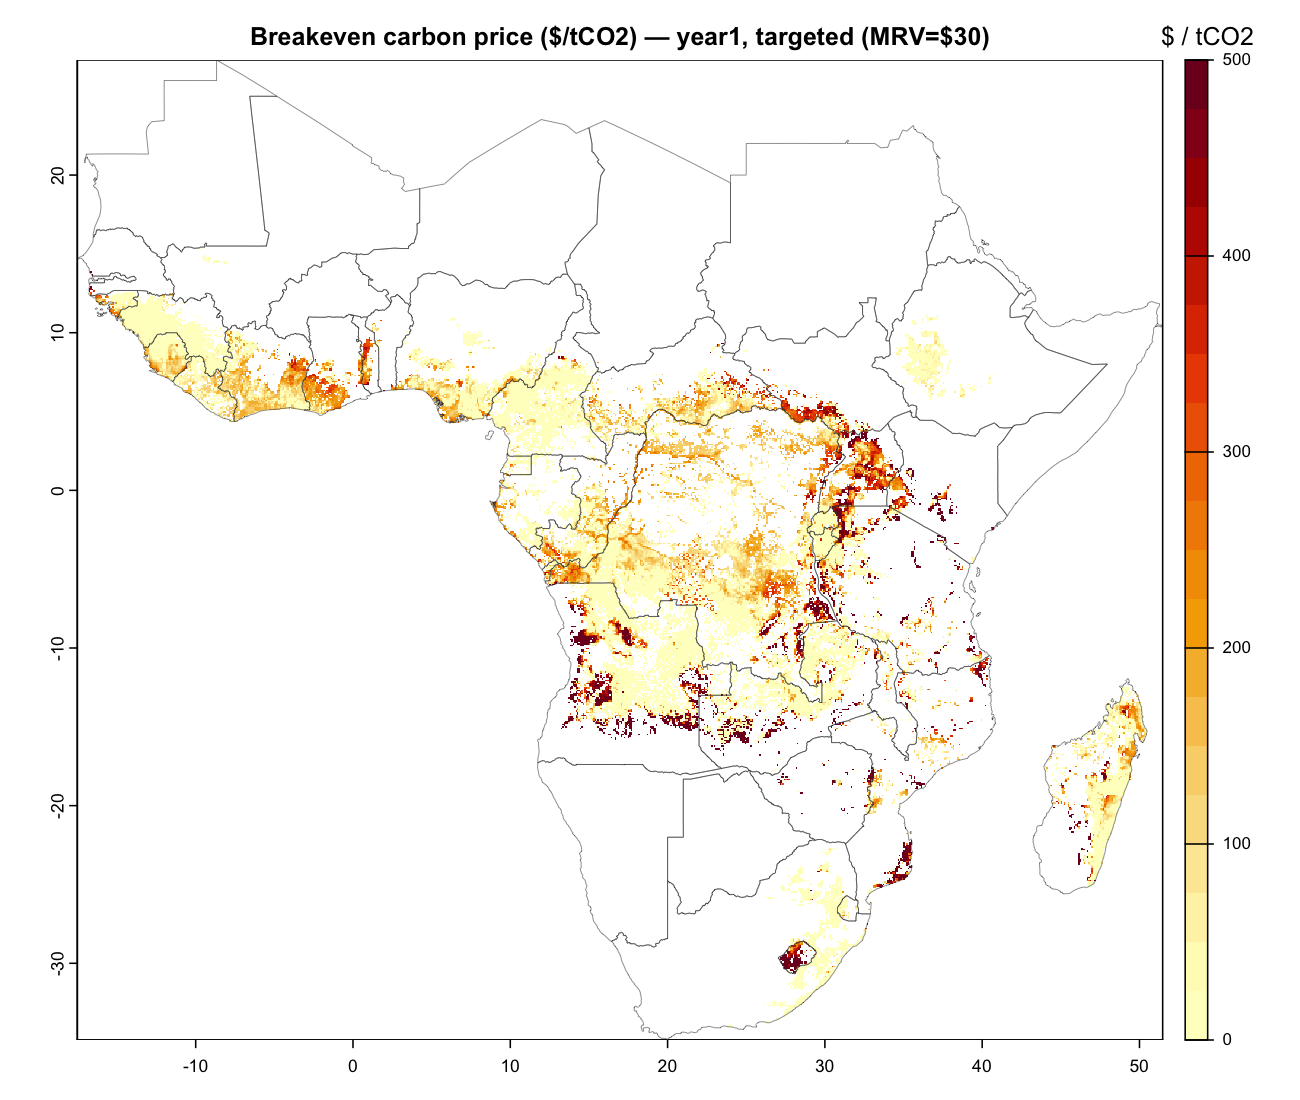
\includegraphics[width=2in,height=\textheight,keepaspectratio]{maps/profitability/breakeven_carbon_year1_targeted.png}
&
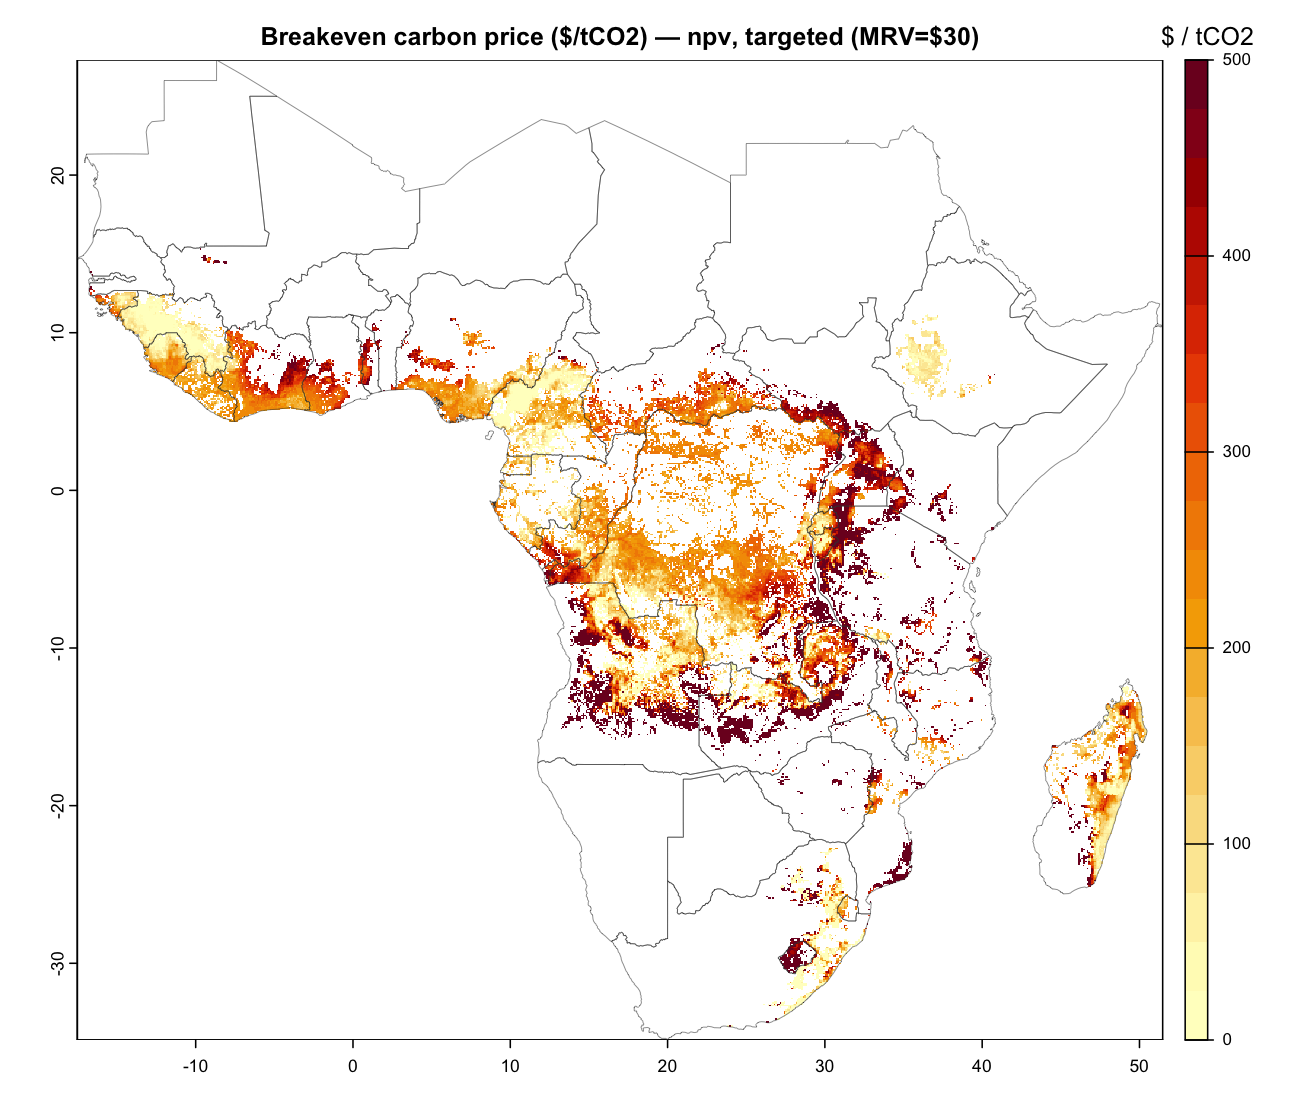
\includegraphics[width=2in,height=\textheight,keepaspectratio]{maps/profitability/breakeven_carbon_npv_targeted.png}
&
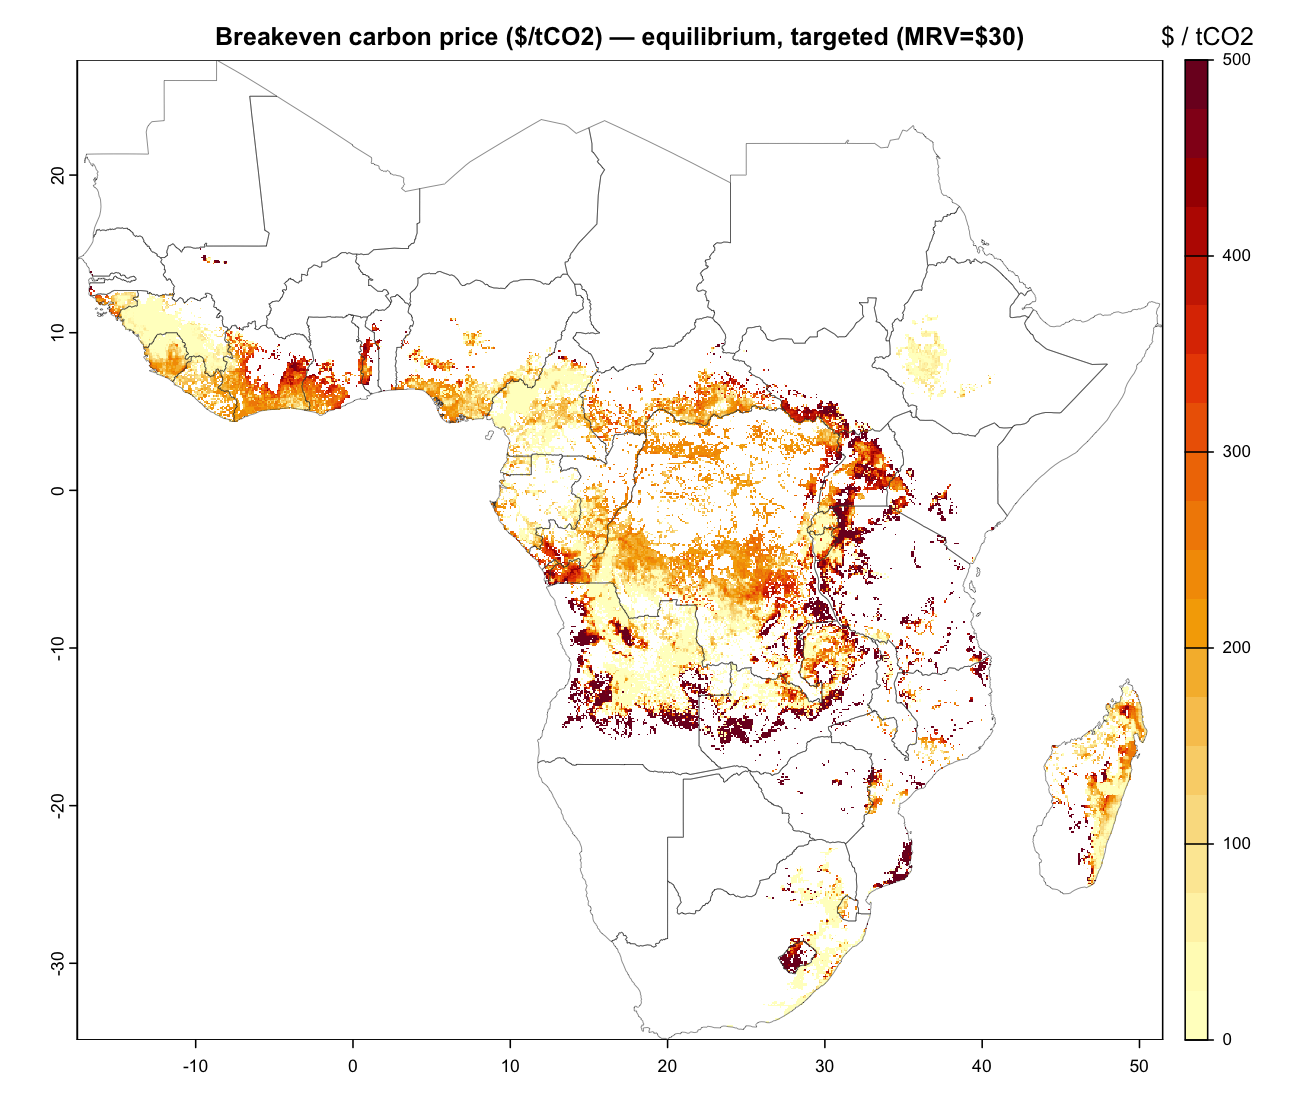
\includegraphics[width=2in,height=\textheight,keepaspectratio]{maps/profitability/breakeven_carbon_equilibrium_targeted.png} \\
\end{longtable}
}

The equilibrium regime tends to need higher carbon prices because the
maintenance dose recurs forever, while year-1 / NPV amortise the
up-front agronomic uplift against a single application.

\begin{center}\rule{0.5\linewidth}{0.5pt}\end{center}

\subsection{4. Per-crop gross margin (selected crops,
targeted)}\label{per-crop-gross-margin-selected-crops-targeted}

The five highest-acreage crops, year-1 and NPV regimes:

{\def\LTcaptype{none} % do not increment counter
\begin{longtable}[]{@{}
  >{\raggedright\arraybackslash}p{(\linewidth - 4\tabcolsep) * \real{0.3333}}
  >{\centering\arraybackslash}p{(\linewidth - 4\tabcolsep) * \real{0.3333}}
  >{\centering\arraybackslash}p{(\linewidth - 4\tabcolsep) * \real{0.3333}}@{}}
\toprule\noalign{}
\begin{minipage}[b]{\linewidth}\raggedright
Crop
\end{minipage} & \begin{minipage}[b]{\linewidth}\centering
Year-1
\end{minipage} & \begin{minipage}[b]{\linewidth}\centering
NPV @ 10 \%
\end{minipage} \\
\midrule\noalign{}
\endhead
\bottomrule\noalign{}
\endlastfoot
Maize (MAIZ) &
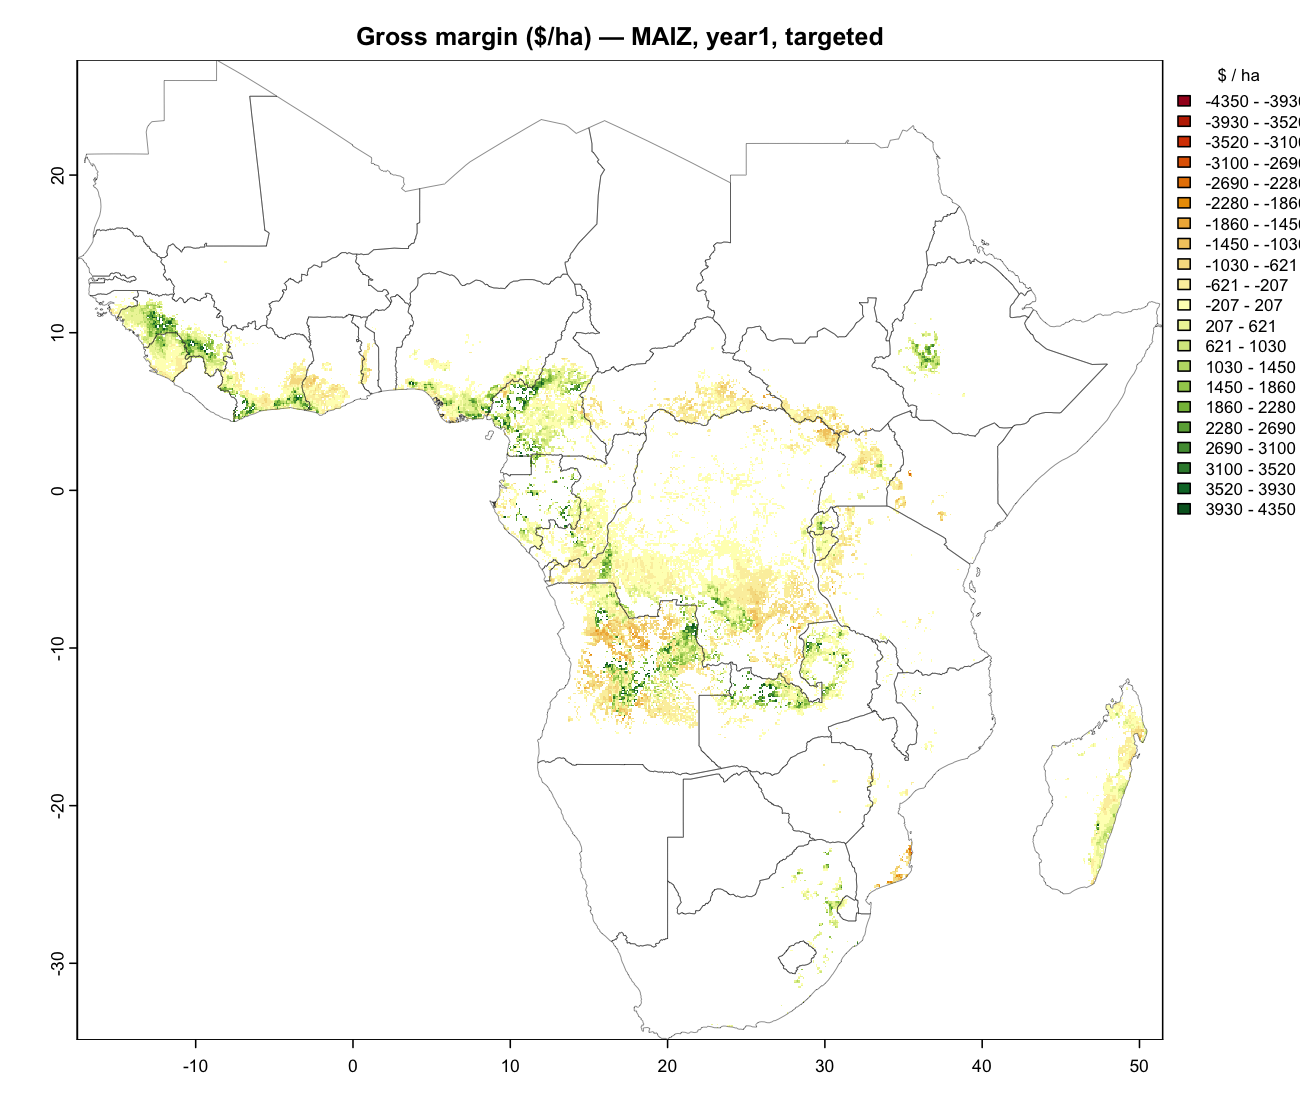
\includegraphics[width=2.4in,height=\textheight,keepaspectratio]{maps/profitability/crop_gm_MAIZ_year1_targeted.png}
&
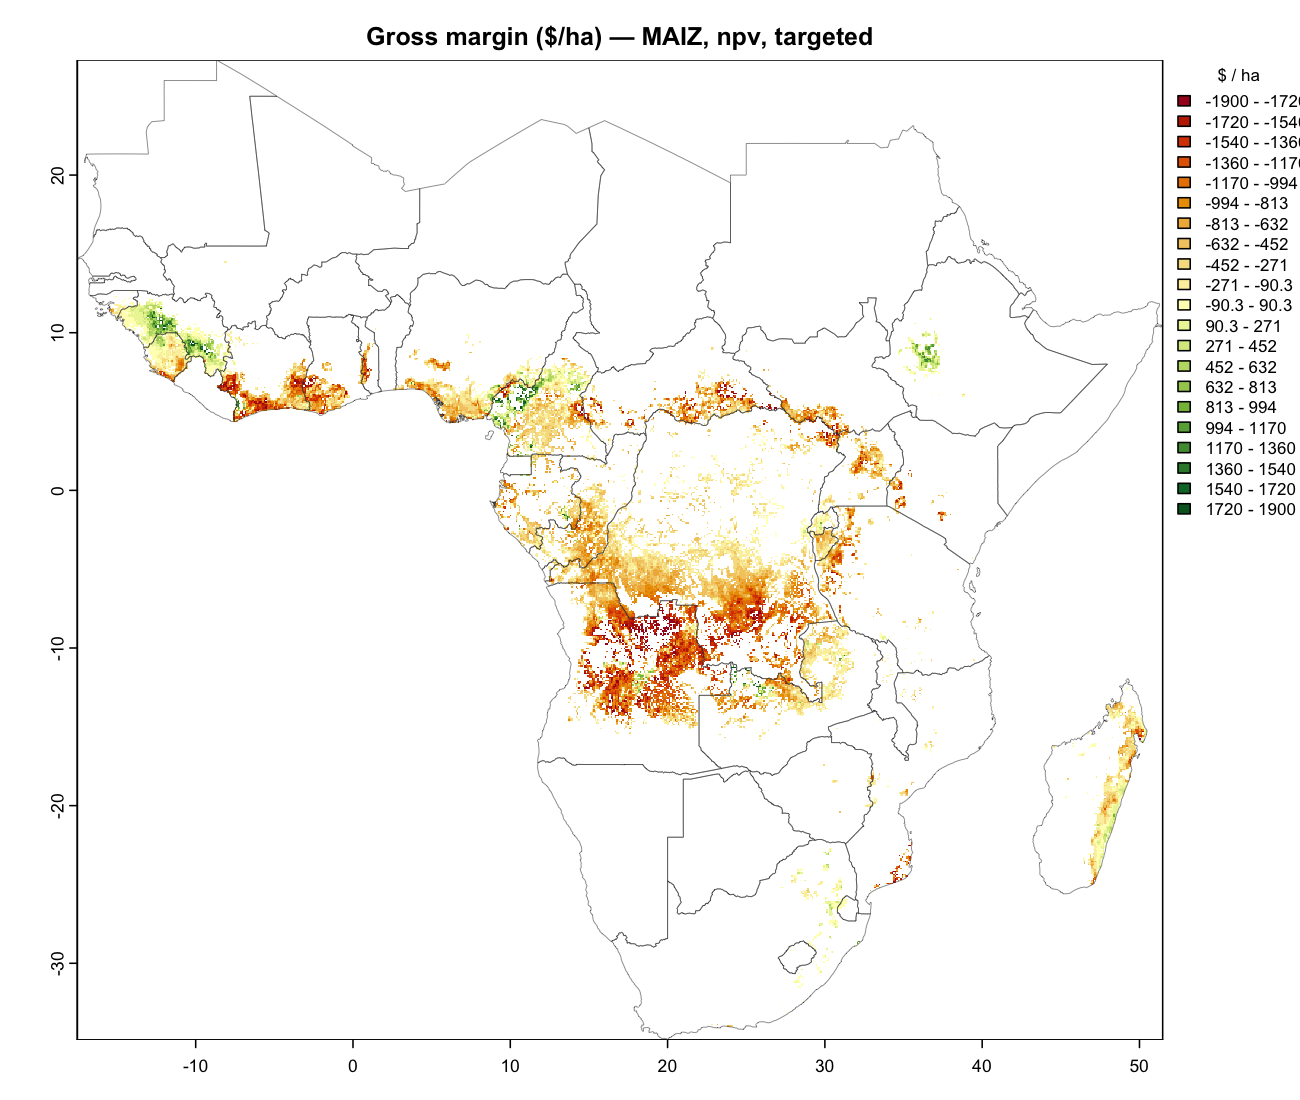
\includegraphics[width=2.4in,height=\textheight,keepaspectratio]{maps/profitability/crop_gm_MAIZ_npv_targeted.png} \\
Sorghum (SORG) &
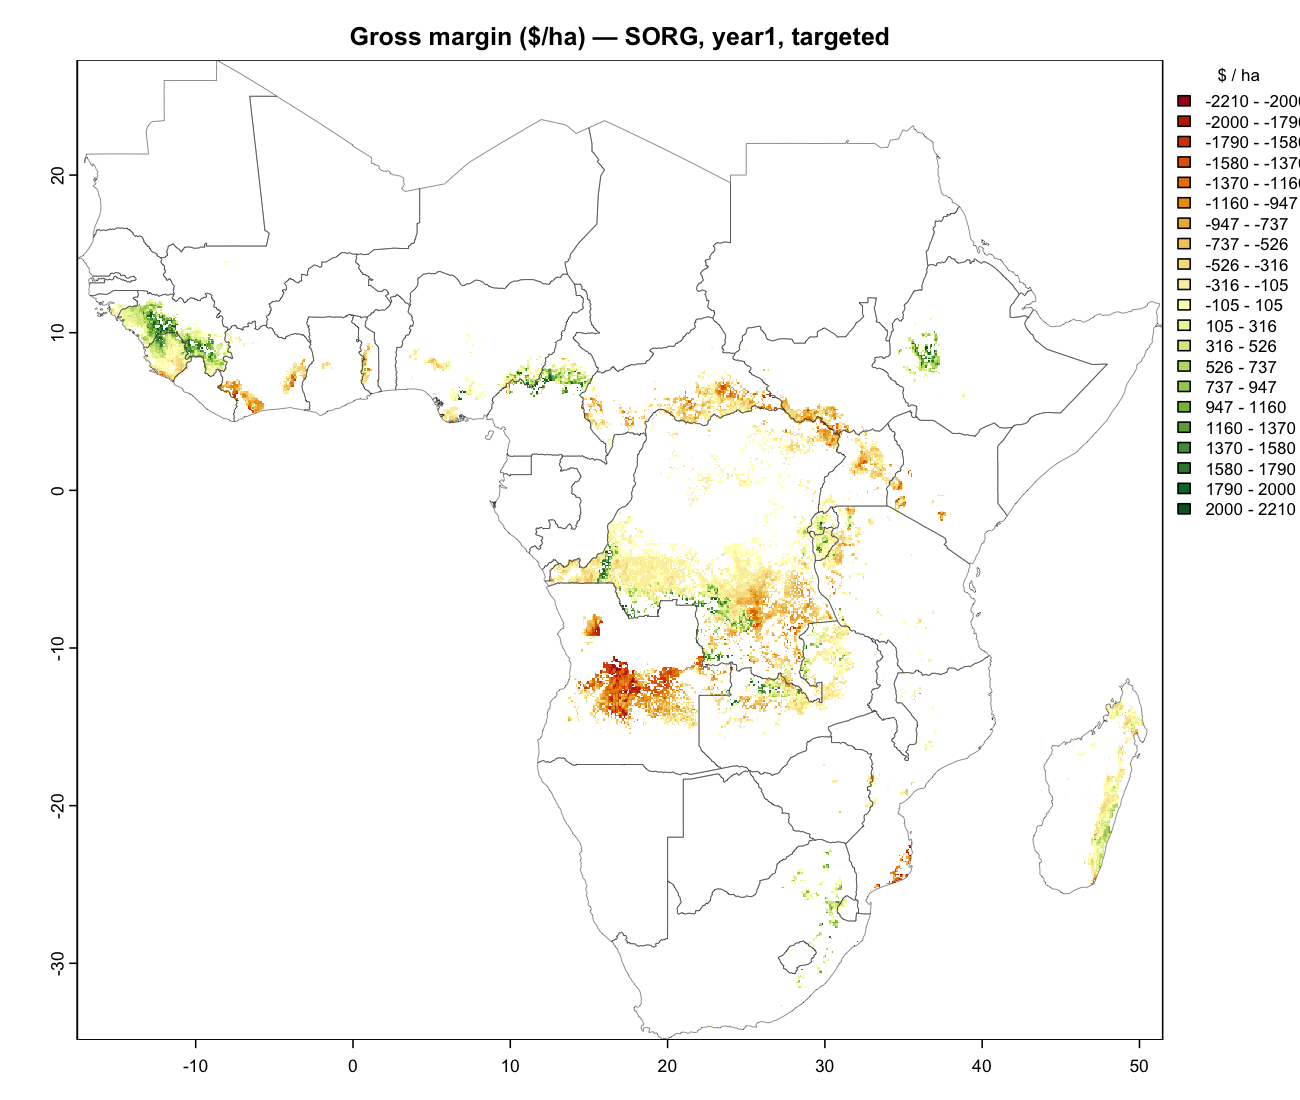
\includegraphics[width=2.4in,height=\textheight,keepaspectratio]{maps/profitability/crop_gm_SORG_year1_targeted.png}
&
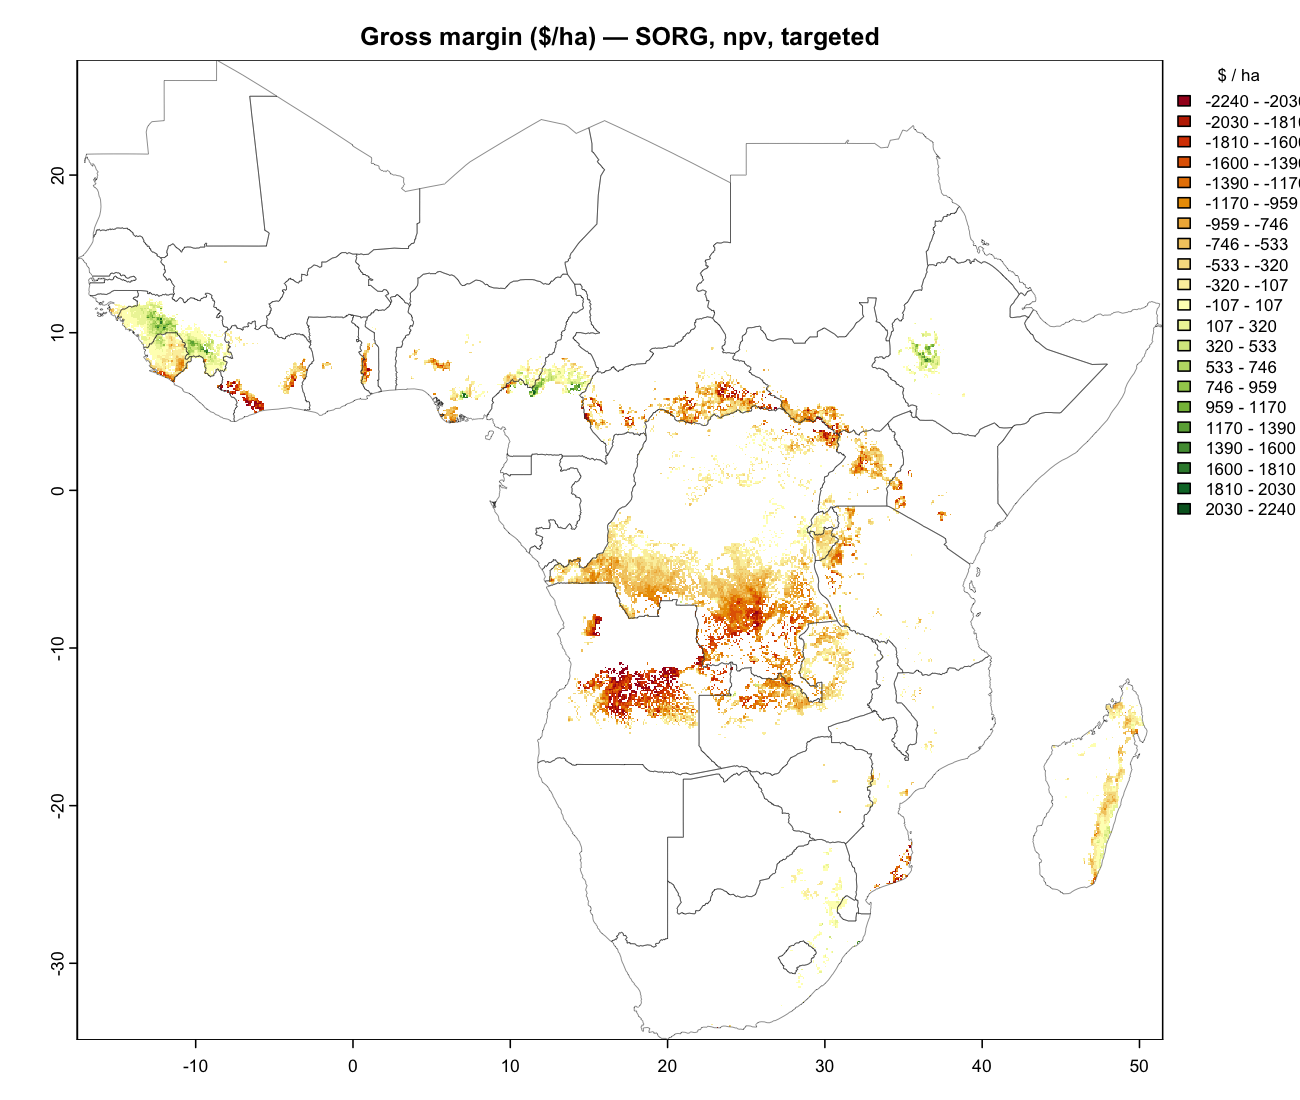
\includegraphics[width=2.4in,height=\textheight,keepaspectratio]{maps/profitability/crop_gm_SORG_npv_targeted.png} \\
Cassava (CASS) &
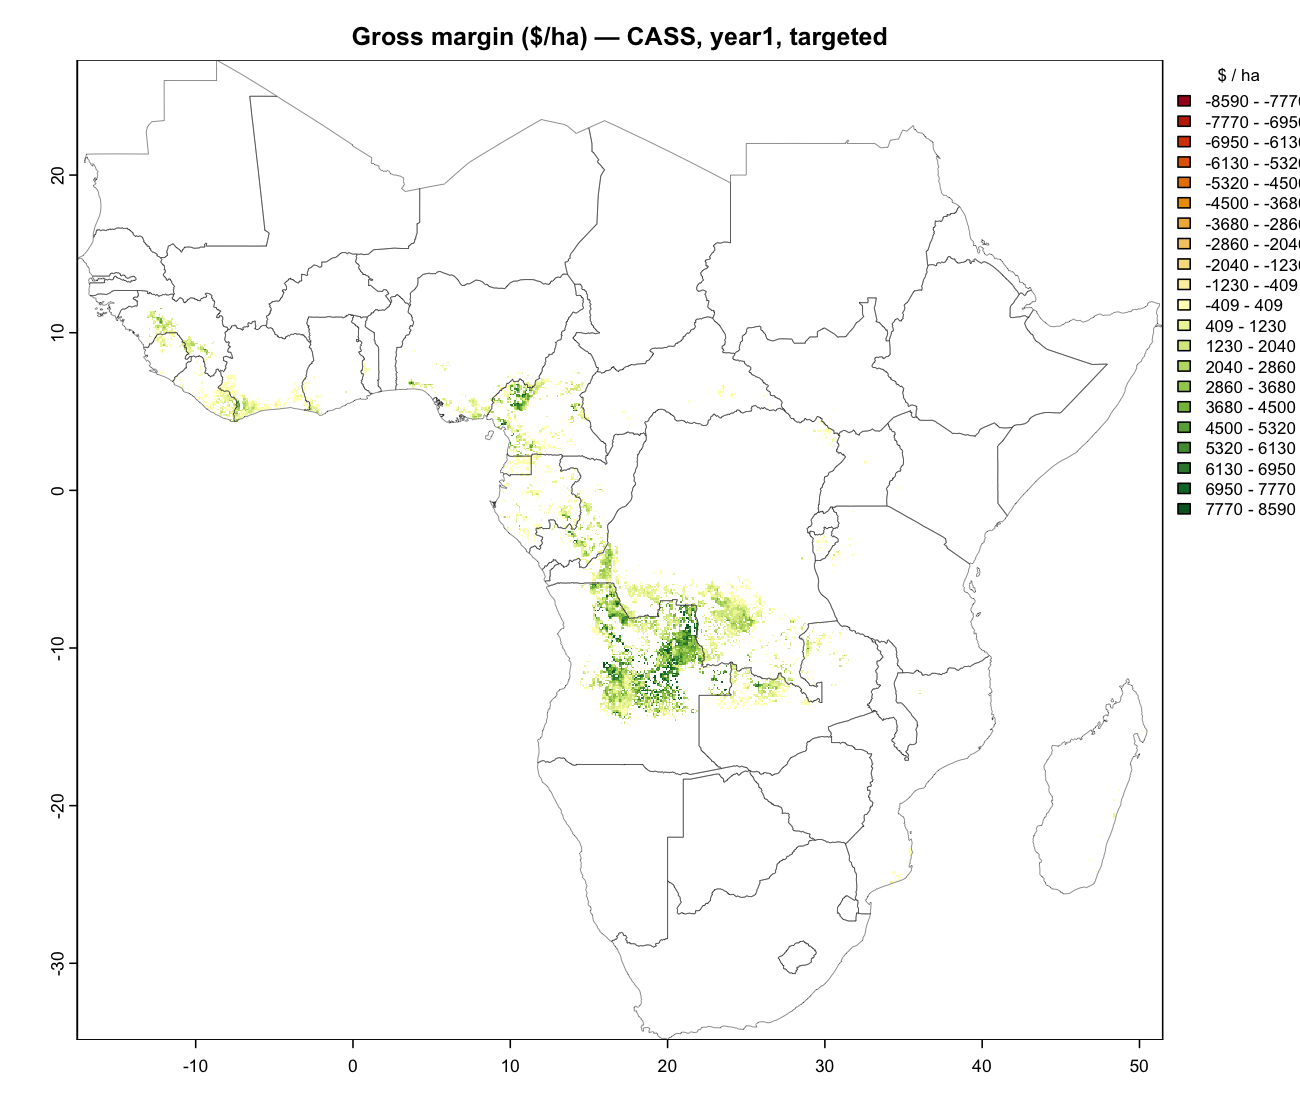
\includegraphics[width=2.4in,height=\textheight,keepaspectratio]{maps/profitability/crop_gm_CASS_year1_targeted.png}
&
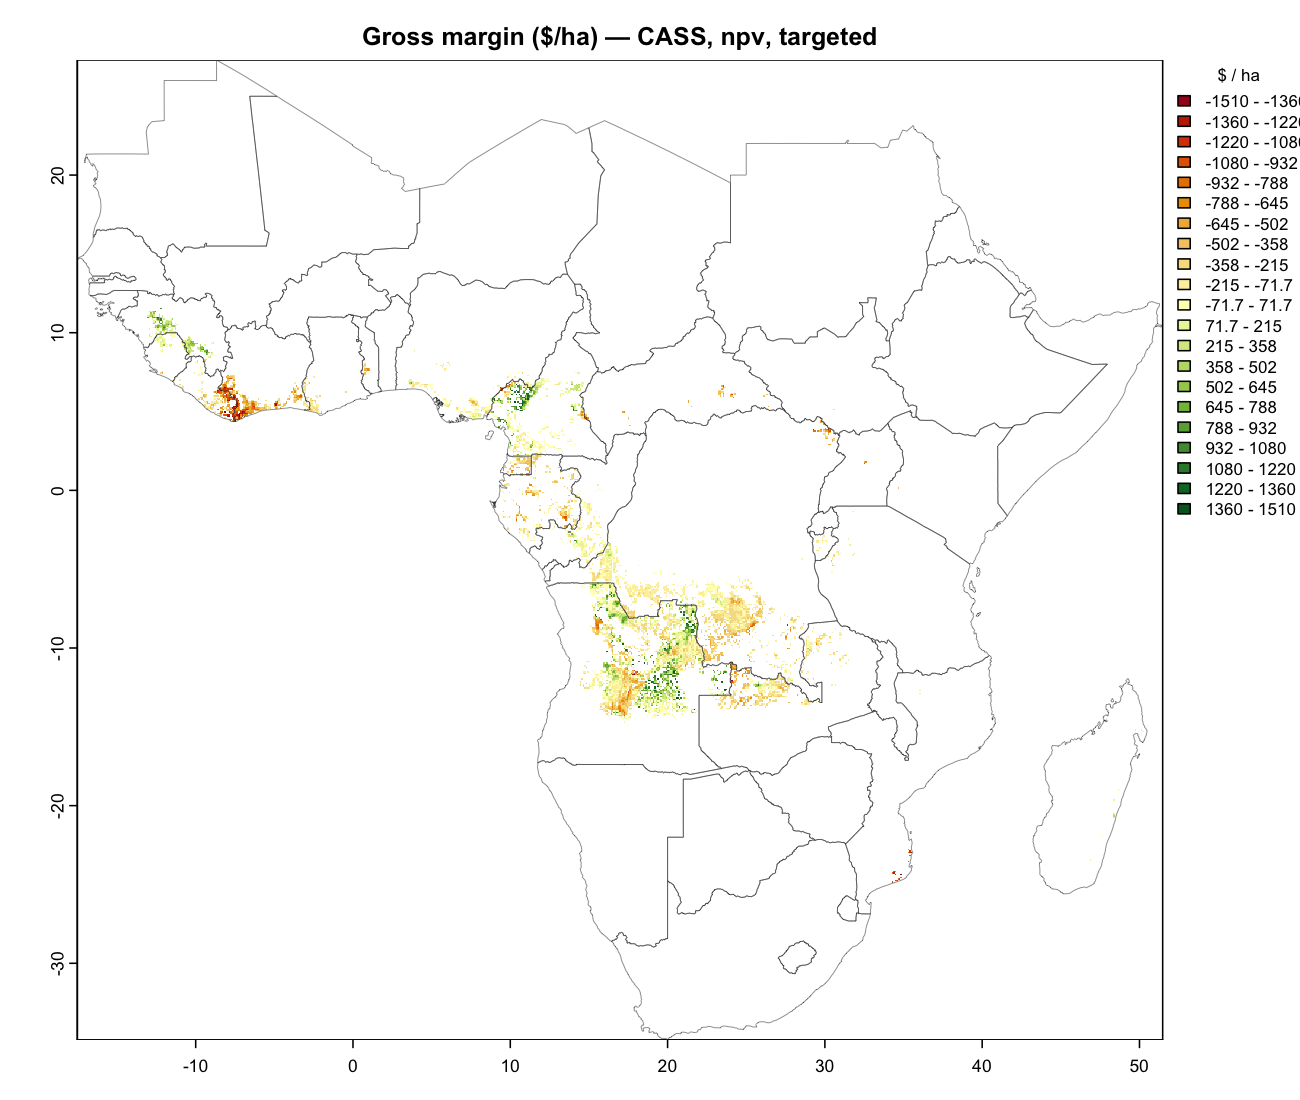
\includegraphics[width=2.4in,height=\textheight,keepaspectratio]{maps/profitability/crop_gm_CASS_npv_targeted.png} \\
Groundnut (GROU) &
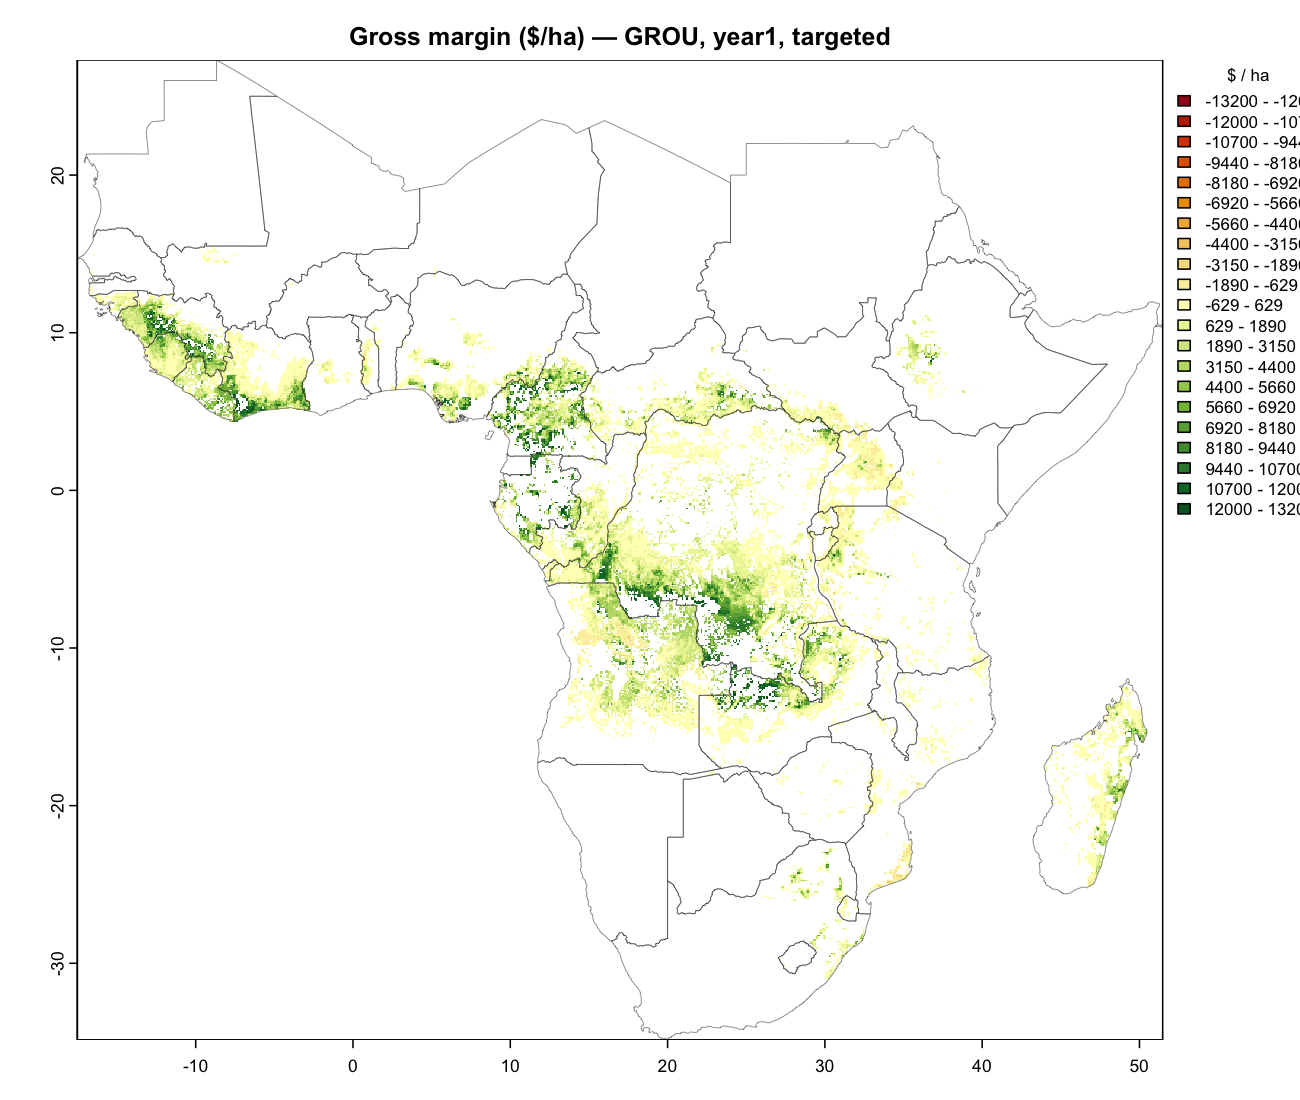
\includegraphics[width=2.4in,height=\textheight,keepaspectratio]{maps/profitability/crop_gm_GROU_year1_targeted.png}
&
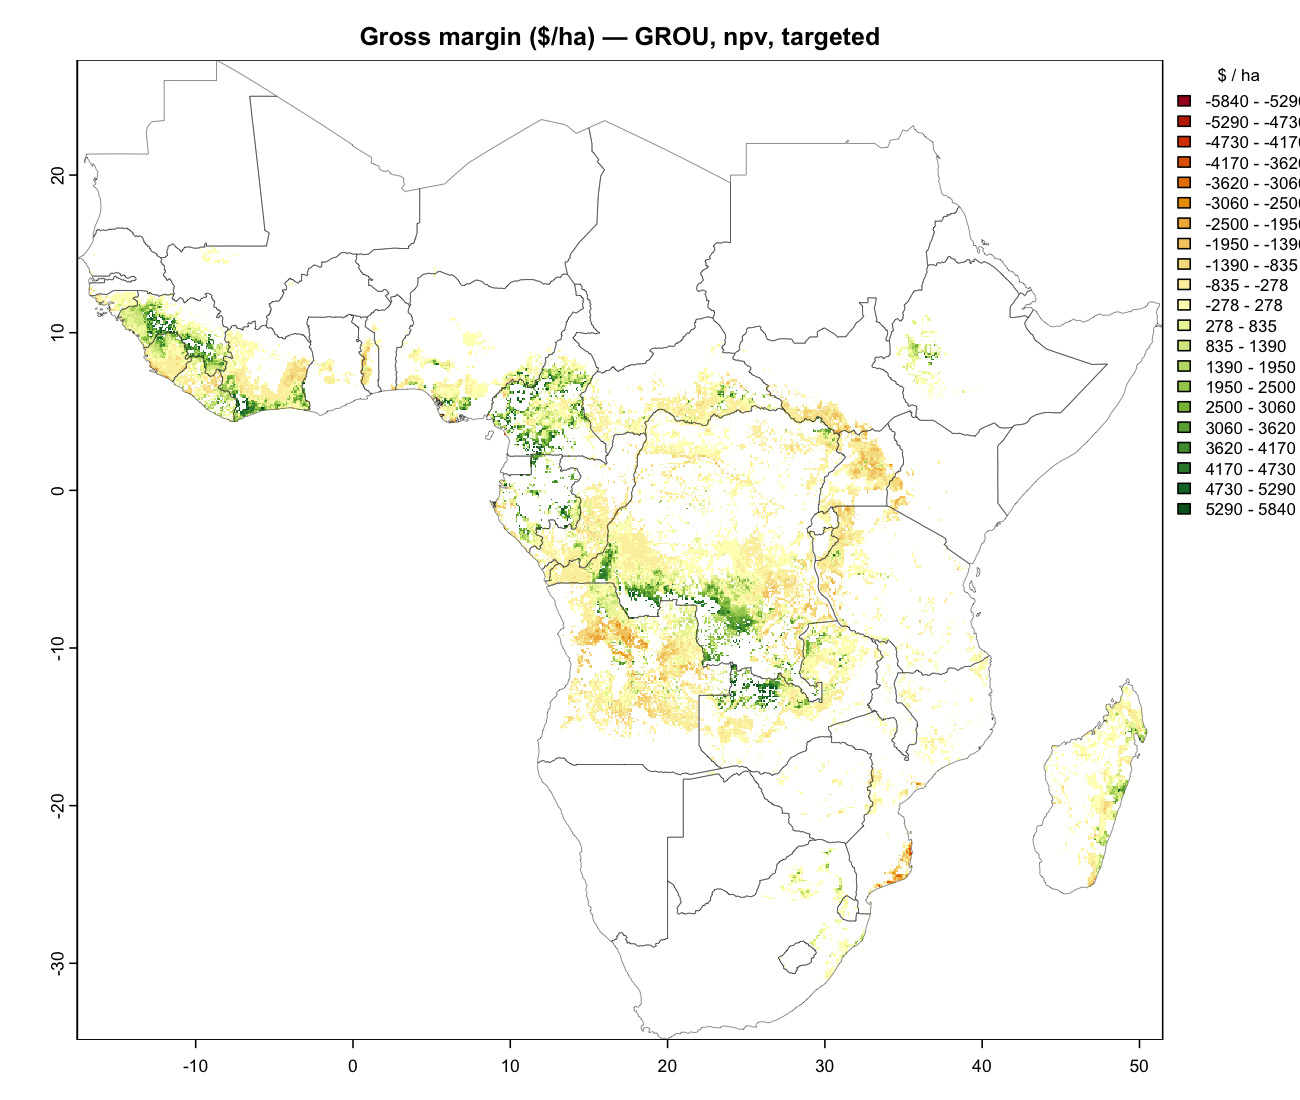
\includegraphics[width=2.4in,height=\textheight,keepaspectratio]{maps/profitability/crop_gm_GROU_npv_targeted.png} \\
Wheat (WHEA) &
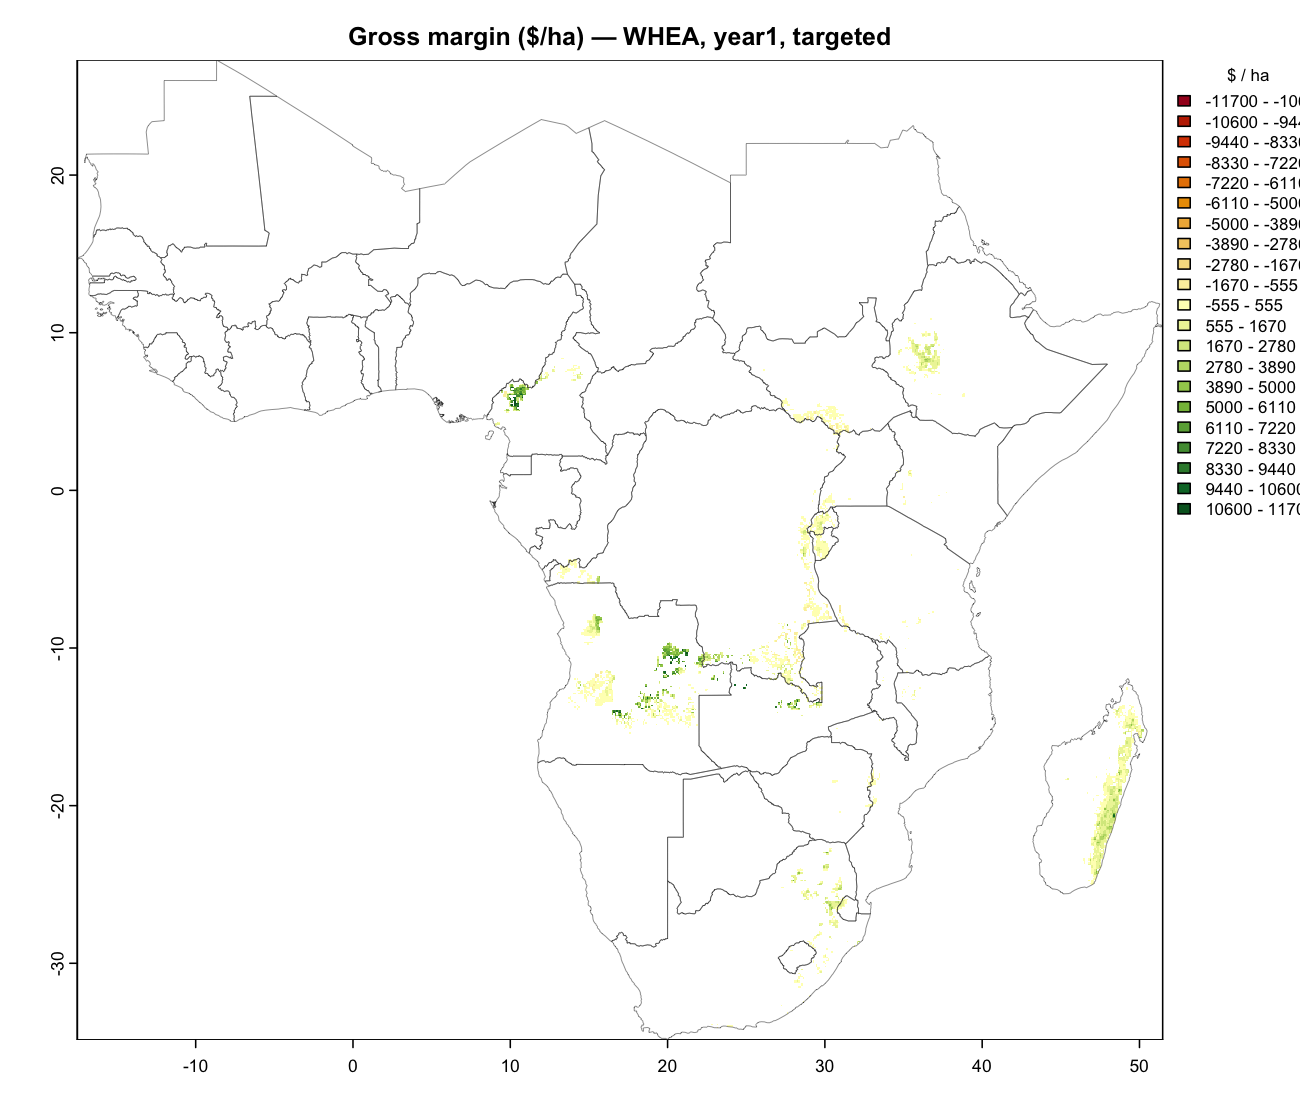
\includegraphics[width=2.4in,height=\textheight,keepaspectratio]{maps/profitability/crop_gm_WHEA_year1_targeted.png}
&
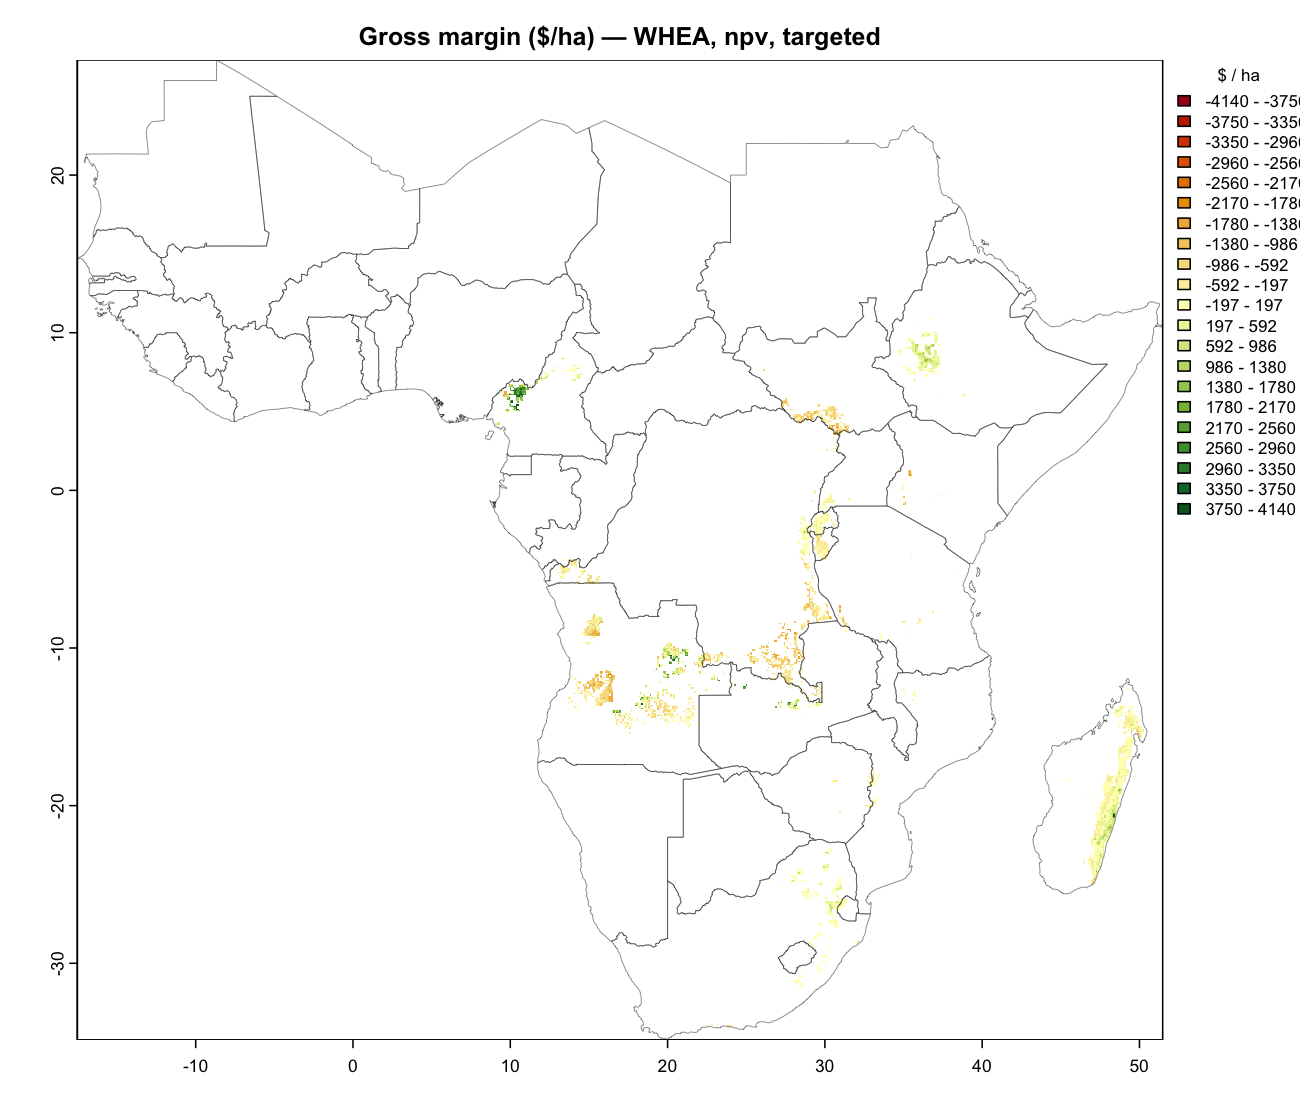
\includegraphics[width=2.4in,height=\textheight,keepaspectratio]{maps/profitability/crop_gm_WHEA_npv_targeted.png} \\
\end{longtable}
}

\begin{center}\rule{0.5\linewidth}{0.5pt}\end{center}

\subsection{5. SSA-wide totals --- one row per regime ×
allocation}\label{ssa-wide-totals-one-row-per-regime-allocation}

Aggregates are summed across all 23 crops, all pixels (no positive-GM
filter unless the column says ``profitable''). Source:
\texttt{docs/tables/output-ssa-summary.csv}.

\begin{small}

{\def\LTcaptype{none} % do not increment counter
\begin{longtable}[]{@{}
  >{\raggedright\arraybackslash}p{(\linewidth - 16\tabcolsep) * \real{0.1111}}
  >{\raggedright\arraybackslash}p{(\linewidth - 16\tabcolsep) * \real{0.1111}}
  >{\raggedleft\arraybackslash}p{(\linewidth - 16\tabcolsep) * \real{0.1111}}
  >{\raggedleft\arraybackslash}p{(\linewidth - 16\tabcolsep) * \real{0.1111}}
  >{\raggedleft\arraybackslash}p{(\linewidth - 16\tabcolsep) * \real{0.1111}}
  >{\raggedleft\arraybackslash}p{(\linewidth - 16\tabcolsep) * \real{0.1111}}
  >{\raggedleft\arraybackslash}p{(\linewidth - 16\tabcolsep) * \real{0.1111}}
  >{\raggedleft\arraybackslash}p{(\linewidth - 16\tabcolsep) * \real{0.1111}}
  >{\raggedleft\arraybackslash}p{(\linewidth - 16\tabcolsep) * \real{0.1111}}@{}}
\toprule\noalign{}
\begin{minipage}[b]{\linewidth}\raggedright
Regime
\end{minipage} & \begin{minipage}[b]{\linewidth}\raggedright
Allocation
\end{minipage} & \begin{minipage}[b]{\linewidth}\raggedleft
Total GM (M\$)
\end{minipage} & \begin{minipage}[b]{\linewidth}\raggedleft
Agro return (M\$)
\end{minipage} & \begin{minipage}[b]{\linewidth}\raggedleft
Basalt cost (M\$)
\end{minipage} & \begin{minipage}[b]{\linewidth}\raggedleft
CDR revenue (M\$)
\end{minipage} & \begin{minipage}[b]{\linewidth}\raggedleft
Total CDR (Mt)
\end{minipage} & \begin{minipage}[b]{\linewidth}\raggedleft
Profitable area (Mha)
\end{minipage} & \begin{minipage}[b]{\linewidth}\raggedleft
CDR on profitable (Mt)
\end{minipage} \\
\midrule\noalign{}
\endhead
\bottomrule\noalign{}
\endlastfoot
year1 & targeted & 18439.6 & 30219.9 & 21545.4 & 10565.7 & 81.27 &
137.87 & 58.41 \\
npv & targeted & -1106.7 & 12029.7 & 21545.4 & 8390.7 & 81.27 & 132.41 &
37.43 \\
equilibrium & targeted & 1965.3 & 6044 & 7363.9 & 3442 & 26.48 & 134.88
& 13.6 \\
year1 & uniform\_10 & 19950.3 & 30219.9 & 75918.2 & 13742.4 & 105.71 &
127.07 & 81.59 \\
npv & uniform\_10 & -6106.2 & 5494.5 & 75918.2 & 10913.5 & 105.71 &
119.24 & 68.31 \\
equilibrium & uniform\_10 & -4200.4 & 6044 & 75918.2 & 13742.4 & 105.71
& 120.61 & 71.02 \\
year1 & uniform\_20 & 9712.2 & 30219.9 & 151836.4 & 27484.8 & 211.42 &
124.08 & 153.67 \\
npv & uniform\_20 & -17701.2 & 5494.5 & 151836.4 & 21827 & 211.42 &
117.41 & 130.4 \\
equilibrium & uniform\_20 & -14438.5 & 6044 & 151836.4 & 27484.8 &
211.42 & 118.64 & 135.36 \\
year1 & uniform\_50 & -21002 & 30219.9 & 379591 & 68712.1 & 528.55 &
120.61 & 355.11 \\
npv & uniform\_50 & -52486.3 & 5494.5 & 379591 & 54567.4 & 528.55 &
116.07 & 314.58 \\
equilibrium & uniform\_50 & -45152.7 & 6044 & 379591 & 68712.1 & 528.55
& 117.09 & 325.44 \\
\end{longtable}
}

\end{small}

\begin{center}\rule{0.5\linewidth}{0.5pt}\end{center}

\subsection{6. Top crops by aggregate gross margin (NPV
regime)}\label{top-crops-by-aggregate-gross-margin-npv-regime}

The full crop × regime × allocation matrix is in
\texttt{docs/tables/output-crop-ranking.csv}. Below: the top eight crops
by total GM under the NPV-targeted scenario.

\begin{small}

{\def\LTcaptype{none} % do not increment counter
\begin{longtable}[]{@{}
  >{\raggedleft\arraybackslash}p{(\linewidth - 8\tabcolsep) * \real{0.2000}}
  >{\raggedright\arraybackslash}p{(\linewidth - 8\tabcolsep) * \real{0.2000}}
  >{\raggedleft\arraybackslash}p{(\linewidth - 8\tabcolsep) * \real{0.2000}}
  >{\raggedleft\arraybackslash}p{(\linewidth - 8\tabcolsep) * \real{0.2000}}
  >{\raggedleft\arraybackslash}p{(\linewidth - 8\tabcolsep) * \real{0.2000}}@{}}
\toprule\noalign{}
\begin{minipage}[b]{\linewidth}\raggedleft
Rank
\end{minipage} & \begin{minipage}[b]{\linewidth}\raggedright
Crop
\end{minipage} & \begin{minipage}[b]{\linewidth}\raggedleft
Total GM (M\$)
\end{minipage} & \begin{minipage}[b]{\linewidth}\raggedleft
Profitable area (Mha)
\end{minipage} & \begin{minipage}[b]{\linewidth}\raggedleft
Total CDR (Mt)
\end{minipage} \\
\midrule\noalign{}
\endhead
\bottomrule\noalign{}
\endlastfoot
1 & BEAN & 1285.63 & 4.749 & 17.142 \\
2 & GROU & 874.78 & 10.537 & 11.838 \\
3 & POTA & 872.05 & 1.408 & 2.793 \\
4 & SWPO & 48.11 & 2.963 & 4.925 \\
5 & LENT & 20.98 & 0.103 & 0.068 \\
6 & WHEA & 14.07 & 2.904 & 0.687 \\
7 & BARL & 6.45 & 1.212 & 0.256 \\
8 & CHIC & 5.2 & 0.41 & 0.114 \\
\end{longtable}
}

\end{small}

\begin{center}\rule{0.5\linewidth}{0.5pt}\end{center}

\subsection{7. Country breakdown --- NPV, targeted (top 12 by
GM)}\label{country-breakdown-npv-targeted-top-12-by-gm}

Full per-country table for all regime × allocation combinations:
\texttt{docs/tables/output-country-summary.csv} (528 rows = 44 countries
× 12 scenarios). Below: the top dozen by aggregate GM in the
NPV-targeted scenario.

\begin{small}

{\def\LTcaptype{none} % do not increment counter
\begin{longtable}[]{@{}rlrrr@{}}
\toprule\noalign{}
Rank & ISO3 & GM (M\$) & Profitable area (Mha) & Total CDR (Mt) \\
\midrule\noalign{}
\endhead
\bottomrule\noalign{}
\endlastfoot
1 & CMR & 3313.11 & 0.843 & 17.56 \\
2 & GIN & 567.24 & 0.561 & 3.974 \\
3 & RWA & 369.48 & 0.418 & 3.121 \\
4 & ETH & 297.15 & 0.654 & 5.271 \\
5 & BDI & 154.63 & 0.275 & 2.109 \\
6 & SLE & 41.2 & 0.112 & 1.526 \\
7 & ZAF & 24.08 & 0.072 & 0.051 \\
8 & GAB & 12.61 & 0.017 & 0.411 \\
9 & SWZ & 0.59 & 0.005 & 0.024 \\
10 & GNQ & -1.17 & 0.009 & 0.196 \\
11 & MDG & -1.27 & 0.1 & 0.813 \\
12 & SEN & -1.56 & 0 & 0.003 \\
\end{longtable}
}

\end{small}

\begin{center}\rule{0.5\linewidth}{0.5pt}\end{center}

\subsection{8. How to rebuild}\label{how-to-rebuild}

\begin{Shaded}
\begin{Highlighting}[]
\CommentTok{\# 1. Make sure erw{-}7 outputs exist}
\FunctionTok{ls}\NormalTok{ data/economics\_erw/targeted/  }\CommentTok{\# should have 69 = 23 crops × 3 regimes}

\CommentTok{\# 2. Render maps + tables}
\ExtensionTok{Rscript}\NormalTok{ erw/erw{-}10{-}profitability{-}maps{-}tables.R}

\CommentTok{\# 3. Rebuild this PDF}
\FunctionTok{bash}\NormalTok{ docs/build{-}erw{-}results.sh}
\end{Highlighting}
\end{Shaded}

The R script is idempotent and \textasciitilde3 min on an M-series
laptop. The PDF build requires \texttt{pandoc} + \texttt{xelatex} (same
toolchain as \texttt{erw-model.pdf}).

\end{document}
